\documentclass[10pt,letterpaper]{article}
\usepackage[top=0.85in,left=1.5in,footskip=0.75in,marginparwidth=1.5in]{geometry}

% use Unicode characters - try changing the option if you run into troubles with special characters (e.g. umlauts)
\usepackage[utf8]{inputenc}

% clean citations
\usepackage{cite}

% hyperref makes references clicky. use \url{www.example.com} or \href{www.example.com}{description} to add a clicky url
\usepackage{nameref,hyperref}

% line numbers
\usepackage[right]{lineno}

% improves typesetting in LaTeX
\usepackage{microtype}
\DisableLigatures[f]{encoding = *, family = * }

% algorithm module
\usepackage{algorithm}
\usepackage[noend]{algpseudocode}

% text layout - change as needed
\raggedright
\setlength{\parindent}{0.5cm}
\textwidth 5.25in 
\textheight 8.75in

% Remove % for double line spacing
%\usepackage{setspace} 
%\doublespacing

% use adjustwidth environment to exceed text width (see examples in text)
\usepackage{changepage}

% adjust caption style
\usepackage[aboveskip=1pt,labelfont=bf,labelsep=period,singlelinecheck=off]{caption}

% remove brackets from references
\makeatletter
\renewcommand{\@biblabel}[1]{\quad#1.}
\makeatother

% headrule, footrule and page numbers
\usepackage{lastpage,fancyhdr,graphicx}
\usepackage{epstopdf}
\pagestyle{myheadings}
\pagestyle{fancy}
\fancyhf{}
\rfoot{\thepage/\pageref{LastPage}}
\renewcommand{\footrule}{\hrule height 2pt \vspace{2mm}}
\fancyheadoffset[L]{2.25in}
\fancyfootoffset[L]{2.25in}
\newcommand{\hl}[2]{{\color{#1}\bfseries [#2]}}
\newcommand{\todo}[1]{\hl{red}{#1}}
% use \textcolor{color}{text} for colored text (e.g. highlight to-do areas)
\usepackage{color}

% define custom colors (this one is for figure captions)
\definecolor{Gray}{gray}{.25}

% this is required to include graphics
\usepackage{graphicx}

% use if you want to put caption to the side of the figure - see example in text
\usepackage{sidecap}

% use for have text wrap around figures
\usepackage{wrapfig}
\usepackage[pscoord]{eso-pic}
\usepackage[fulladjust]{marginnote}
\usepackage{amsmath}
\usepackage{amssymb}
\usepackage{amsthm}

\newtheorem{theorem}{Theorem}[section]
\newtheorem{corollary}{Corollary}[theorem]
\newtheorem{lemma}[theorem]{Lemma}
\DeclareMathOperator*{\argmax}{arg\,max}
\DeclareMathOperator*{\argmin}{arg\,min}

\reversemarginpar

% document begins here
\begin{document}
\vspace*{0.35in}

% title goes here:
\begin{flushleft}
{\Large
\textbf\newline{Yet another correlation analysis of mutation score, fault detection, and test suite size}
}
\newline
% authors go here:
\\
CSE 599 course porject, Yiqun Chen\textsuperscript{1,*}\\
Supervisor: Ren\'e Just \\

\bigskip
\bf{1} University of Washington, Seattle
% \\
% \bf{2} Affiliation B
\\
\bigskip
*yiqunc@uw.com
\end{flushleft}


% now start line numbers
% \linenumbers

% the * after section prevents numbering
\section*{Abstract}
Finding best practice in test creation has been an active research area for software engineering domain for decades. A good test suite, by definition, should detect real faults. However the target of interest is usually unknown to the programmers a priori, which prompts the use of mutants, which are artifically generated faults. Mutation score based testing uses mutants as proxies for measuring strength of a test suite, and recently researchers have made multiple attempts to validate the merit of mutant score based testing strategy. This report aims to look at the relationship between fault detection, mutation scores, and size of test suites systematically and investigate a few claims made by Papadakis et al. Specifically, they argued that while mutation score is highly correlated with fault detection, the correlation decreases after adjusting for test suite sizes. This observation leads to their conclusion of test suite size being a confounder, and the aim of this report is to demonstrate both conceputal and statistical analysis pitfalls in their work and offer alternative measures of correlation.




\section{Introduction}


This paper repeats and refutes the recent result from Papadakis et al. To answer the question of whether mutation scores are really indicative of real fault detection probability, they conducted a series of correlation based analysis and logistic regression modeling. 

They report a drastic drop of correlation between fault detection and mutation scores after  
The major claims of their paper can be broken down as the following:
\begin{itemize}
\item
Claim 1: Correlation between mutation score and real fault detection is induced by a confounding variable, test suite size. 

\item
Claim 2: Both mutation score and test suite size are statistically singnificant predictors of real fault detection, but both are not very practically significant.
\item
Claim 3: Prioritizing test suites with higher mutation scores leads to an improved real fault detection compared to random selection.

\end{itemize}

For the remainder of the report, we will focus on investigating claim 1 and 2 and answer the following research questions (RQ):

\begin{itemize}
\item
RQ 1: Are the results presented to support claim 1 in the original paper reproducible? If so, how sensitive are the results to choices of parameters such as sampling ratio, normalization of mutation scores, and etc.
\item
RQ 2: Controlling for test suite size explicitly is just a poor man's version of many statistical techniques such as multivariate regression or partial correlation. Given that the maximal Pearson correlation between a continuous variable and a binary variable is less than 1, would the same results hold for other measures of correlation? 


\item
RQ 3: It's well-known that correlation doesn't imply causation; however, it's often neglected that a decrease of correlation after stratifying on a variable does not make the stratifying vairable a confounder. We instead propose the concept of coupling and a plausible causal pathway to formalize the idea of causality in this case.

\end{itemize}




\subsection{Terminology} 

Before moving on to the constructive section of the paper, we first introduce a list of terms we will use for the rest of discussion, many of which will be illustrated using the kill matrix example in Table \ref{tab:coupling}. 


\begin{table}[ht!]
\captionsetup{justification=centering}
\begin{center}
\begin{tabular}{c c c c c c c}
\hline
\multicolumn{1}{c}{Test} & \multicolumn{1}{c}{Real Fault} & \multicolumn{5}{c}{Mutants} \\
\hline
% \cmidrule{3-7}
      & $f$ & $m_1$ & $m_2$ & $m_3$ & $m_4$  \\
\hline
$t_1$ &  1  &   1   &   1   &   0   &   0   &    \\
$t_2$ &  0  &   0   &   1   &   0   &   0   &    \\
$t_3$ &  0  &   0   &   0   &   1   &   0  &    \\
\hline
\end{tabular}
\caption{Example Test-mutant matrix (kill matrix)} \label{tab:coupling}
\end{center}
\end{table}


\begin{itemize}
    \item 
    Project: refers to the class of Java programs used in the study (Chart, Closure, Lang, Math, Time)
    \item
    Task: individual bugs studied ($n=231$)
    \item
    (Real) fault: a single bug unique to each task. 
    \item
    Fault detection (FD): we say a test suite detects the fault (equivalently FD=1) if at least one of the tests detects the fault. For instance, the suite $\{t_1,t_2,t_3\}$ detects the fault since $f=1$ for $t_1$, but the subset $\{t_2,t_3\}$ does not detect the fault (FD=0).
    
    \item
    Mutation score (MS): 
    \begin{itemize}
        \item 
        for a given suite of mutants $\mathcal{M}$, the un-normalized mutation score for a test suite $T$ on $\mathcal{M}$ is total number of mutants detected by the individual tests. 
        For instance, consider $\mathcal{M} = \{m_1,m_2,m_3,m_4\}$ and $T= \{t_1,t_2\}$, then the un-normalized mutation score would be 2 since $m_1$ and $m_2$ are detected.
        \item
        
        for a given suite of mutants $\mathcal{M}$, the normalized mutation score for a test suite on $\mathcal{M}$ is the ratio of total number of mutants detected by the individual tests, divided by total number of detectable mutants by this test suite. Again, consider  $\mathcal{M} = \{m_1,m_2,m_3,m_4\}$ and $T= \{t_1,t_2\}$, the normalized mutation score would be $\frac{2}{3}$ since $m_4$ cannot be detected by any tests in the entire test pool ($t_1,t_2,t_3$).
        
    \end{itemize}
    
    
    \item
    Size of a test suite: number of tests in the suite. 
    
    \item
    For a collection of tests $T$ or mutants $\mathcal{M}$, we use $|T|$ or $|\mathcal{M}|$ to denote the cardinality of the set
    \item
    For a given real fault, tests in a suite can be categorized into either fault triggering  or non-triggering. We use $G$ to denote the subset of tests that detects the fault.

    \item
    Coupling probability: for a given test suite $T$, a fault $f$, and a mutant $m$, the coupling probability of a mutant to a real fault (we will suppress the dependence on $T$ for notational convenience) is defined to be:
    
\begin{equation}
P_{m,f} = P(t \text{ detects } f | t \text{ detects } m), t\stackrel{\text{Uniform}}{\sim} T
\end{equation}

For instance, if we consider $T=\{t_1,t_2,t_3\}$ and fault $f$ in Table \ref{tab:coupling}, $P_{m_1,f}= 1  $ and $P_{m_2,f} = \frac{1}{2}$. As for mutants that are not detected at all such as $m_4$, we use the convention that $P_{m_4,f} = 0$.

\item 
Estimating coupling probability: 
for any existing test suite $T_0 \subset T$, one can estimate this probability by its empirical counterpart:
\begin{equation}
\hat{P}_{m,f} =  \frac{\hat{P}(t \text{ detects } m \text{ and } f )}{\hat{P}(t \text{ detects } m)}
\end{equation} 

\item
Perfect coupling: we say a mutant $m$ is perfectly coupled to a fault $f$ if $P_{m,f}= 1$. Specifically note that this coincides with the familiar concept of coupling in the literature if one consider the test suite $T$ to be all the tests of interest. For instance, if we consider $T = \{t_1,t_2,t_3\}$, $m_1$ and $f$ are perfectly coupled.


\item
Perfect de-coupling: we say a mutant $m$ is perfectly de-coupled to a fault $f$ if $P_{m,f}= 0$ but $P(m \text{ detected }) > 0$. For instance, if we consider $T = \{t_1,t_2,t_3\}$, $m_3$ and $f$ are perfectly de-coupled but $m_4$ is not.

\item
Probabilistic coupling:  we say a mutant $m$ is probablistically coupled to a fault $f$ if $P_{m,f}\in (0,1)$.


\item
Pearson correlation: for any two given random variables $X,Y$, Pearson correlation is defined to be 
\begin{equation}
    Cor(X,Y) = \rho_{X,Y} = \frac{\mathbf{E}[(X-\mathbf{E}X)(Y-\mathbf{E}Y)]}{\sqrt[]{Var(X)Var(Y)}}
\end{equation}
 where $\mathbf{E}$ denotes the expectation and $Var(\cdot)$ denotes the variance of a random variable. Specifically note that Pearson correlation is always bounded between [-1,1] and attains the upper/lower bound only if $Y$ is a linear function of $X$. 
\item
Empirical Pearson correlation: in practice we just take empirical average and variance to obtain the estimated correlation,
\begin{equation}
    \hat{Cor}(X,Y) = \hat{\rho}_{X,Y} = \frac{\sum_{i=1}^N[(X_i-\bar{X})(Y_i-\bar{Y}]}{\sqrt[]{(\sum_{i=1}^N(X_i-\bar{X})^2)(\sum_{i=1}^N(Y_i-\bar{Y})^2)}}
\end{equation} where $\bar{X} = \frac{1}{N}\sum_{i=1}^N X_i$.

\item
Partial correlation: we will only discuss partial correlation for 3 random variables in this report but in general, partial correlation (abbreviated as $PCor$) measures the association between two random variables with with the effect of a set of controlling random variables removed. It is similar to adding a controlling variable in multiple regression but provides a measure of the strength of relationship, instead of effect size. 

Consider three random variables $X,Y,Z$ where $Z$ is the control variable. Then partial correlation of $X$ and $Y$ after controlling for $Z$ can be expressed numerically as:
\begin{equation}
PCor_Z(X,Y) =\rho_{X,Y|Z}= \frac{\rho_{X,Y}-\rho_{X,Z}\cdot \rho_{Y,Z}}{\sqrt[]{(1-\rho_{X,Z}^2)(1-\rho_{Y,Z}^2)}}
\end{equation}

The intuition for partial correlation is that we are looking at the correlation between $X$ and $Y$ after removing the linear effect of $Z$ in both variables. Consider an extreme example where  both $X$ and $Y$ are linear functions of $Z$, then they have Pearson correlation of $\pm 1$. However, after removing the linear trend of $Z$, the resulting partial correlation will be 0.



\item
Odds ratio: consider the following logistic regression models
\begin{equation}
    logit(P(FD=1)) = \beta_0 + \beta_1 \cdot MS
\end{equation} and 
\begin{equation}
    logit(P(FD=1)) = \beta^*_0 + \beta^*_1 \cdot MS + \beta^*_2 \cdot Size
\end{equation}
where $logit(x) = \log(\frac{x}{1-x}),x\in [0,1]$.

\begin{itemize}
    \item
    Unadjusted odds ratio for $MS$: $e^{\beta_1}$

    
    \item
    
     Adjusted odds ratio for $MS$: $e^{\beta^*_1}$
    
\end{itemize}




\end{itemize}



\section{Method}


\subsection{Sampling mechanisms}
In this section, we introduce the following two sampling mechanisms for generating datasets. While the original paper used uniform 0-20\% sampling for what they call ``random" dataset and used 0.025-50\%, with 2.5\%  
spacing for generating ``fixed" datasets, we decide to change the limit for the latter to 20\% as well. The original paper does not mention any difficulties encountered during sampling but we note that when the sampling ratio is high ($>10-20\%$ for most tasks ), every sampled suite will almost always have at least one test that detects the fault and makes it impossible to compute statistics of interest.

%%% sampling models
\begin{algorithm}
\caption{Generating random size datasets}\label{alg:random_size}
\begin{algorithmic}[1]
\Procedure{RandomSize}{Test suite $T$, Lower bound (LB) = $0$,Upper bound (UB) = $0.2$, $N= 10,000$}
\State ResultList  = []
\For{$i=1,\cdots, N$}
\State $R_i \sim Uniform(LB,UB)$
\State $N_i =\lceil R_i \cdot |T| \rceil$
\State Sample $N_i$ numbers without replacement from $\{1,2,\cdots, |T|\}$
\State Append to ResultList the sampled subset of rows $T_{N_i}$.
\EndFor
\State \textbf{return} ResultList
\EndProcedure
\end{algorithmic}
\end{algorithm}


\begin{algorithm}
\caption{Generating fixed size datasets}\label{alg:random_size}
\begin{algorithmic}[1]
\Procedure{RandomSize}{Test suite $T$, Sampling ratio $R$, $N= 10,000$}
\State ResultList  = []
\For{$i=1,\cdots, N$}
\State $N_i =\lceil R \cdot |T| \rceil$
\State Sample $N_i$ numbers without replacement from $\{1,2,\cdots, |T|\}$
\State Append to ResultList the sampled subset of rows $T_{N_i}$.
\EndFor
\State \textbf{return} ResultList
\EndProcedure
\end{algorithmic}
\end{algorithm}

In practice, we compute and record fault detection, mutation score, and size in each random samples for downstream analysis.

We provide below two examples where we listed only 3 out of 10,000 rows in a returned data frame.

\begin{table}[ht!]
\captionsetup{justification=centering}
\begin{center}
\begin{tabular}{c c c c c c c}
\hline
\multicolumn{1}{c}{Task} & \multicolumn{1}{c}{Fault detection} & \multicolumn{1}{c}{Mutation score} &   \multicolumn{1}{c}{Size}  \\
\hline
% % \cmidrule{3-7}
%       & $f$ & $m_1$ & $m_2$ & $m_3$ & $m_4$  \\
% \hline
Chart-1 &  1  &  300   &   893    \\
Chart-1 &  1  &   312  &   1085        \\
Chart-1 &  1  &   286 &   943      \\
\hline
\end{tabular}
\caption{An example for  test suites generated from a random size approach } \label{tab:random_sample}
\end{center}
\end{table}

\begin{table}[ht!]
\captionsetup{justification=centering}
\begin{center}
\begin{tabular}{c c c c c c c}
\hline
\multicolumn{1}{c}{Task} & \multicolumn{1}{c}{Fault detection} & \multicolumn{1}{c}{Mutation score} &   \multicolumn{1}{c}{Size}  \\
\hline
% % \cmidrule{3-7}
%       & $f$ & $m_1$ & $m_2$ & $m_3$ & $m_4$  \\
% \hline
Chart-1 &  1  &  299   &   930    \\
Chart-1 &  1  &   300  &   930        \\
Chart-1 &  1  &   327 &   930      \\
\hline
\end{tabular}
\caption{An example for  test suites generated from a fixed size approach (with sampling ratio  $= 15\%$)} \label{tab:fixed_sample}
\end{center}
\end{table}



\subsection{Statistical methods}

We consider the following methods, some of which are used in the original paper while the rest are proposals from our own. 


\subsubsection{(Partial) correlation}


Consider a sampled dataset with random size (e.g. Table \ref{tab:random_sample}), we compute the following correlation quantities:

\begin{itemize}
    \item 
    $\hat{\rho}_{MS,FD} $  and  $\hat{\rho}_{MS,FD|Size} $
    \item
     $\hat{\rho}_{Size,FD} $ and $\hat{\rho}_{Size,FD|MS} $
\end{itemize}

Since for each fixed size samples, there is no variation in the size variable, we can only compute $\hat{\rho}_{MS,FD}$ and $\hat{\rho}_{MS,FD|Size}=\hat{\rho}_{MS,FD} $ in this case.

The intuition is that if partial correlation drops significantly compared to the marginal correlation, we have some confidence that the third variable size (or MS) plays a role in the effect of MS (or size) to real fault detection. Note that this is an extension to the correlation presented by the authors since they only compared the correlation computed with random size versus correlation computed with fixed size, which, as we will see in a bit, is a potentially misleading effect size measure.

\subsubsection{Linear regression}

We fit the following linear regression models to assess the effect size of mutation score on fault detection:

\begin{itemize}
    \item 
    Unadjusted:  $P(FD=1) = \beta_0 + \beta_1 \cdot MS$, with random size sampling
    \item
     Adjusted:   $P(FD=1) = \beta^*_0 + \beta^*_1 \cdot MS + \beta^*_2 \cdot Size$,with random size sampling
     \item
     Fixed size: $P(FD=1) = \tilde{\beta}_0 + \tilde{\beta}_1 \cdot MS$, with fixed size sampling
\end{itemize}

A natural comparison in this case will just be comparing the value of $\beta_1,\beta^*_1,$ and $\tilde{\beta}_1$. Since the adjusted regression analysis is essentially stratifying on size, we expect $\beta^*_1$ to be close to $\tilde{\beta}_1$ for a range of sampling ratio. If the unadjusted regression coefficient is much larger than the adjusted one, intuitively one would expect that a lot of association between MS and FD can be attributed to size. 

\subsubsection{Logistic regression}


We fit the following logistic regression models to assess the effect size of mutation score on fault detection:

\begin{itemize}
    \item 
    Unadjusted:  $logit(P(FD=1)) = \beta_0 + \beta_1 \cdot MS$, with random size sampling
    \item
     Adjusted:   $logit(P(FD=1)) = \beta^*_0 + \beta^*_1 \cdot MS + \beta^*_2 \cdot Size$,with random size sampling
     \item
     Fixed size: $logit(P(FD=1)) = \tilde{\beta}_0 + \tilde{\beta}_1 \cdot MS$, with fixed size sampling
\end{itemize}

Similar to the linear regression case, a natural comparison in this case will just be comparing the value of $e^{\beta_1},e^{\beta^*_1},$ and $e^{\tilde{\beta}_1}$ (the exponential of regression coefficient is also referred to as estimated odds ratios and is a popular way to summarize the association between a continuous/binary variable and a binary outcome).  Again, since the adjusted regression analysis is essentially stratifying on size, we expect $e^{\beta^*_1}$ to be close to $e^{\tilde{\beta}_1}$ for a range of sampling ratio.  



\section{Results}

\subsection{Replicating the original paper}

In this final report, due to space and time constraint, we did not put together a separate replication study. This, however, will be one of the to-do items for next steps. 

    \begin{figure}[ht!]
        \centering
        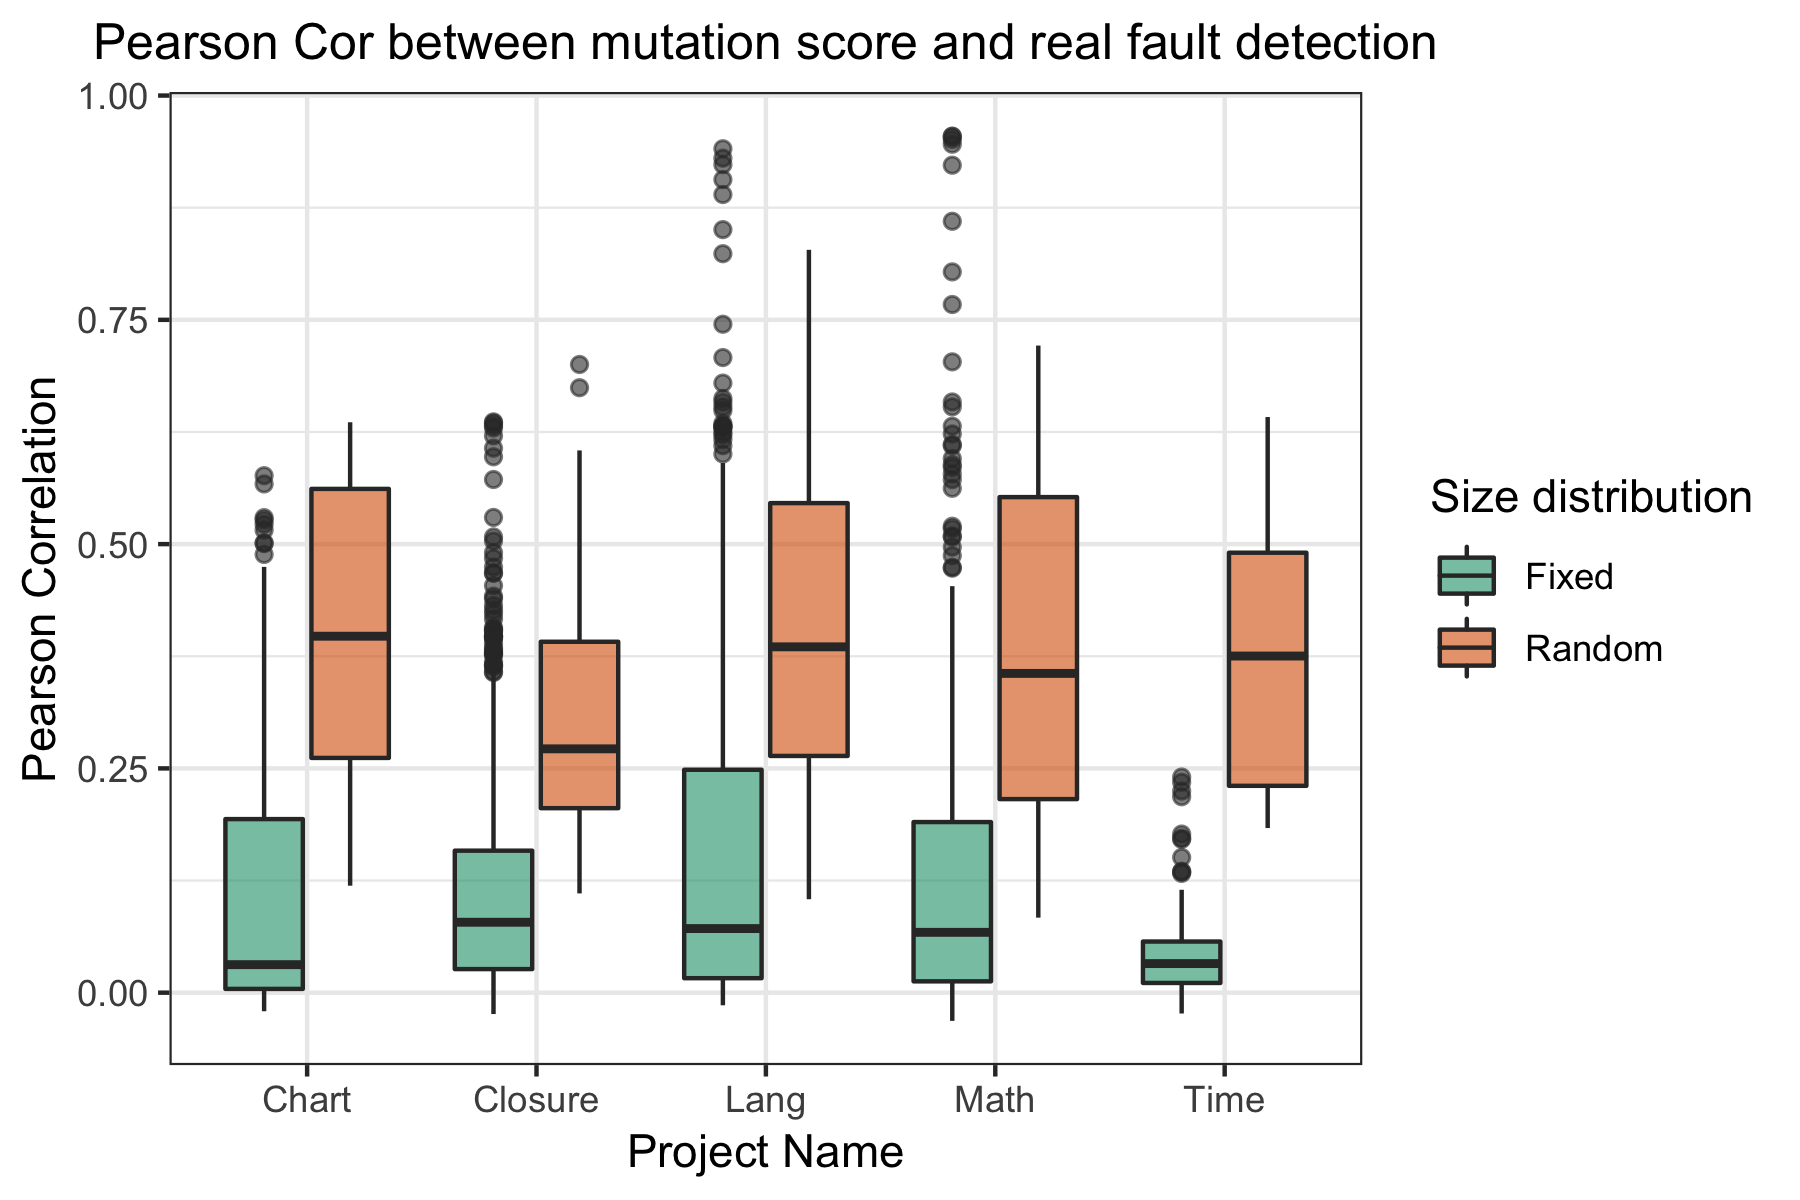
\includegraphics[scale=0.15]{figures/reproduce_fig_3.png}
        \caption{Comparing correlations between mutation score and real fault detection for random and fixed size sampling}
        \label{fig:rep_fig3}
    \end{figure}
    
We provide a ``replication" of Table 3 in the original paper with un-normalized mutation scores instead of normalized ones (See Figure \ref{fig:rep_fig3}). we see that the same trend indeed holds, i.e., the random size sampling produces much higher correlation than the aggregated fixed size correlation. This piece of evidence underpins the essence of their claim that size is a confounder and mutation score is in fact not as correlated with real fault detection as previous scholars thought.



\subsection{Extended correlation analysis}

While controlling for size explicitly using an equally spaced sampling approach, we argue that one should consider the concept of partial correlation directly, which accounts for the linear effect of a potentially confounding variable (e.g. size in the original study). In addition to the partial correlation of MS and FD controlling for size, we also consider the partial correlation of size and FD controlling for MS. 

Note that for some of the datasets due to the imbalance in the outcome (virtually all samples will detect the fault), one cannot compute correlation between fault detection and mutation score and we excluded these in our analyses below.


The motivation for the latter analysis is to quantify the effect of mutant score when considering the correlation of size and fault detection, which is neglected and would be revealing: due to the lack of causal framework, in the previous studies, a confounder is established using the phenomenon of reduced correlation. However, if the same effect is shown in size as well, by the same  logic, we would arrive at the conclusion that mutation score is a confounding variable in the causal path from test suite size to fault detection as well. However, these two claims cannot be simultaneously true and reveal a fundamental shortcoming in the 2015 paper: causation is not equal to correlation and a causal pathway should come from reasoning with domain knowledge instead of being generated with data.     

  \begin{figure}[ht!]
        \centering
        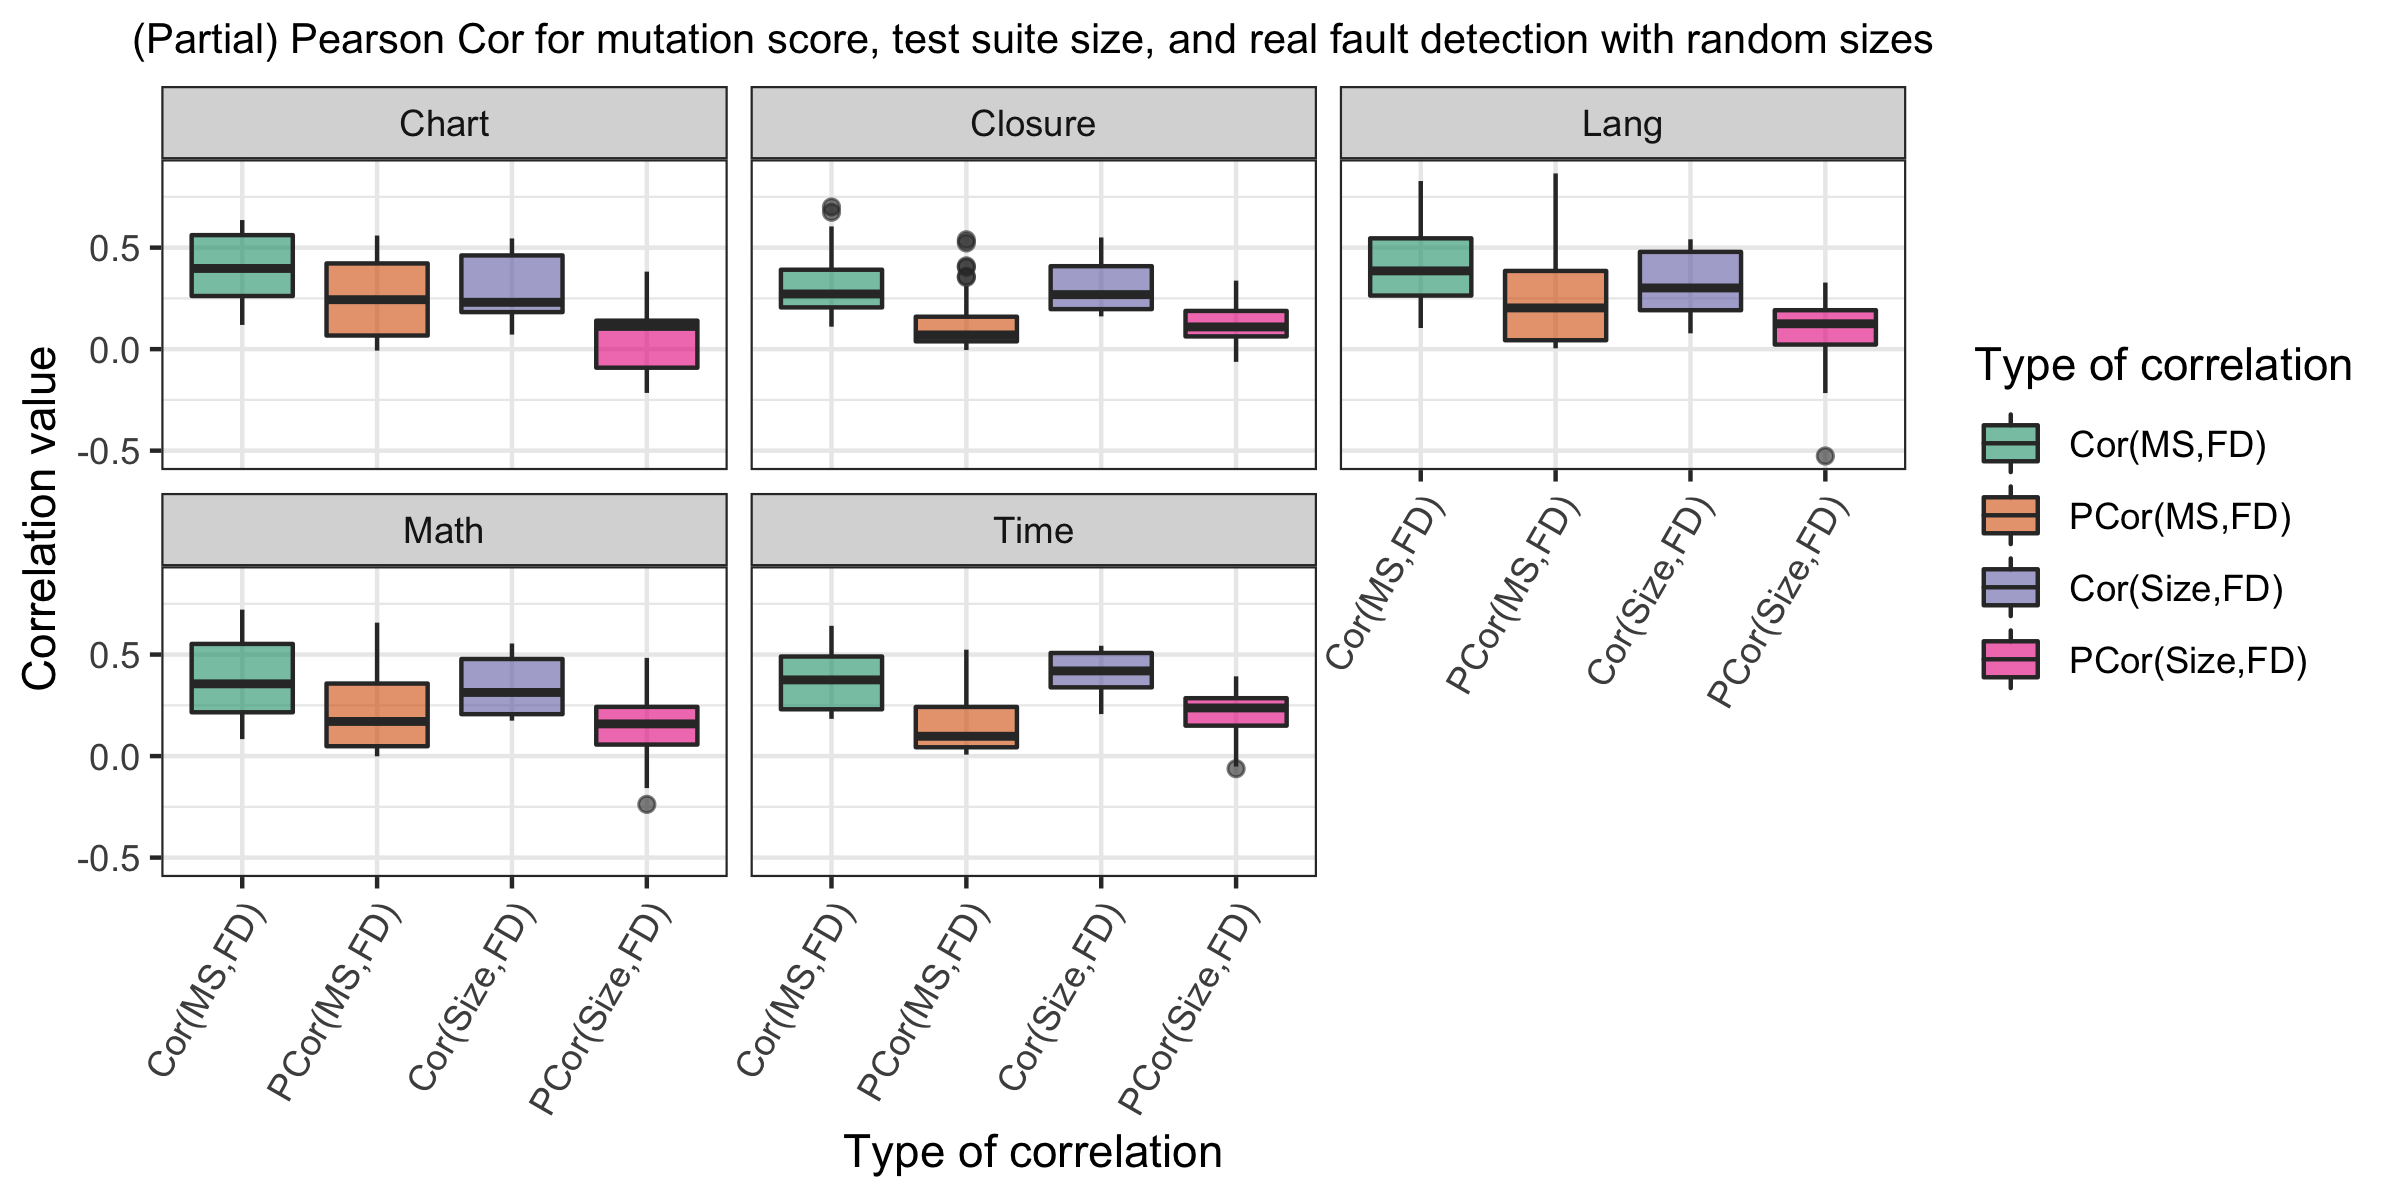
\includegraphics[scale=0.15]{figures/partial_cor_plot.png}
        \caption{Comparing all four (partial) correlations for (mutant score,fault detection) and (test suite size, fault detection) }
        \label{fig:all_4_cor}
    \end{figure}

  \begin{figure}[ht!]
        \centering
        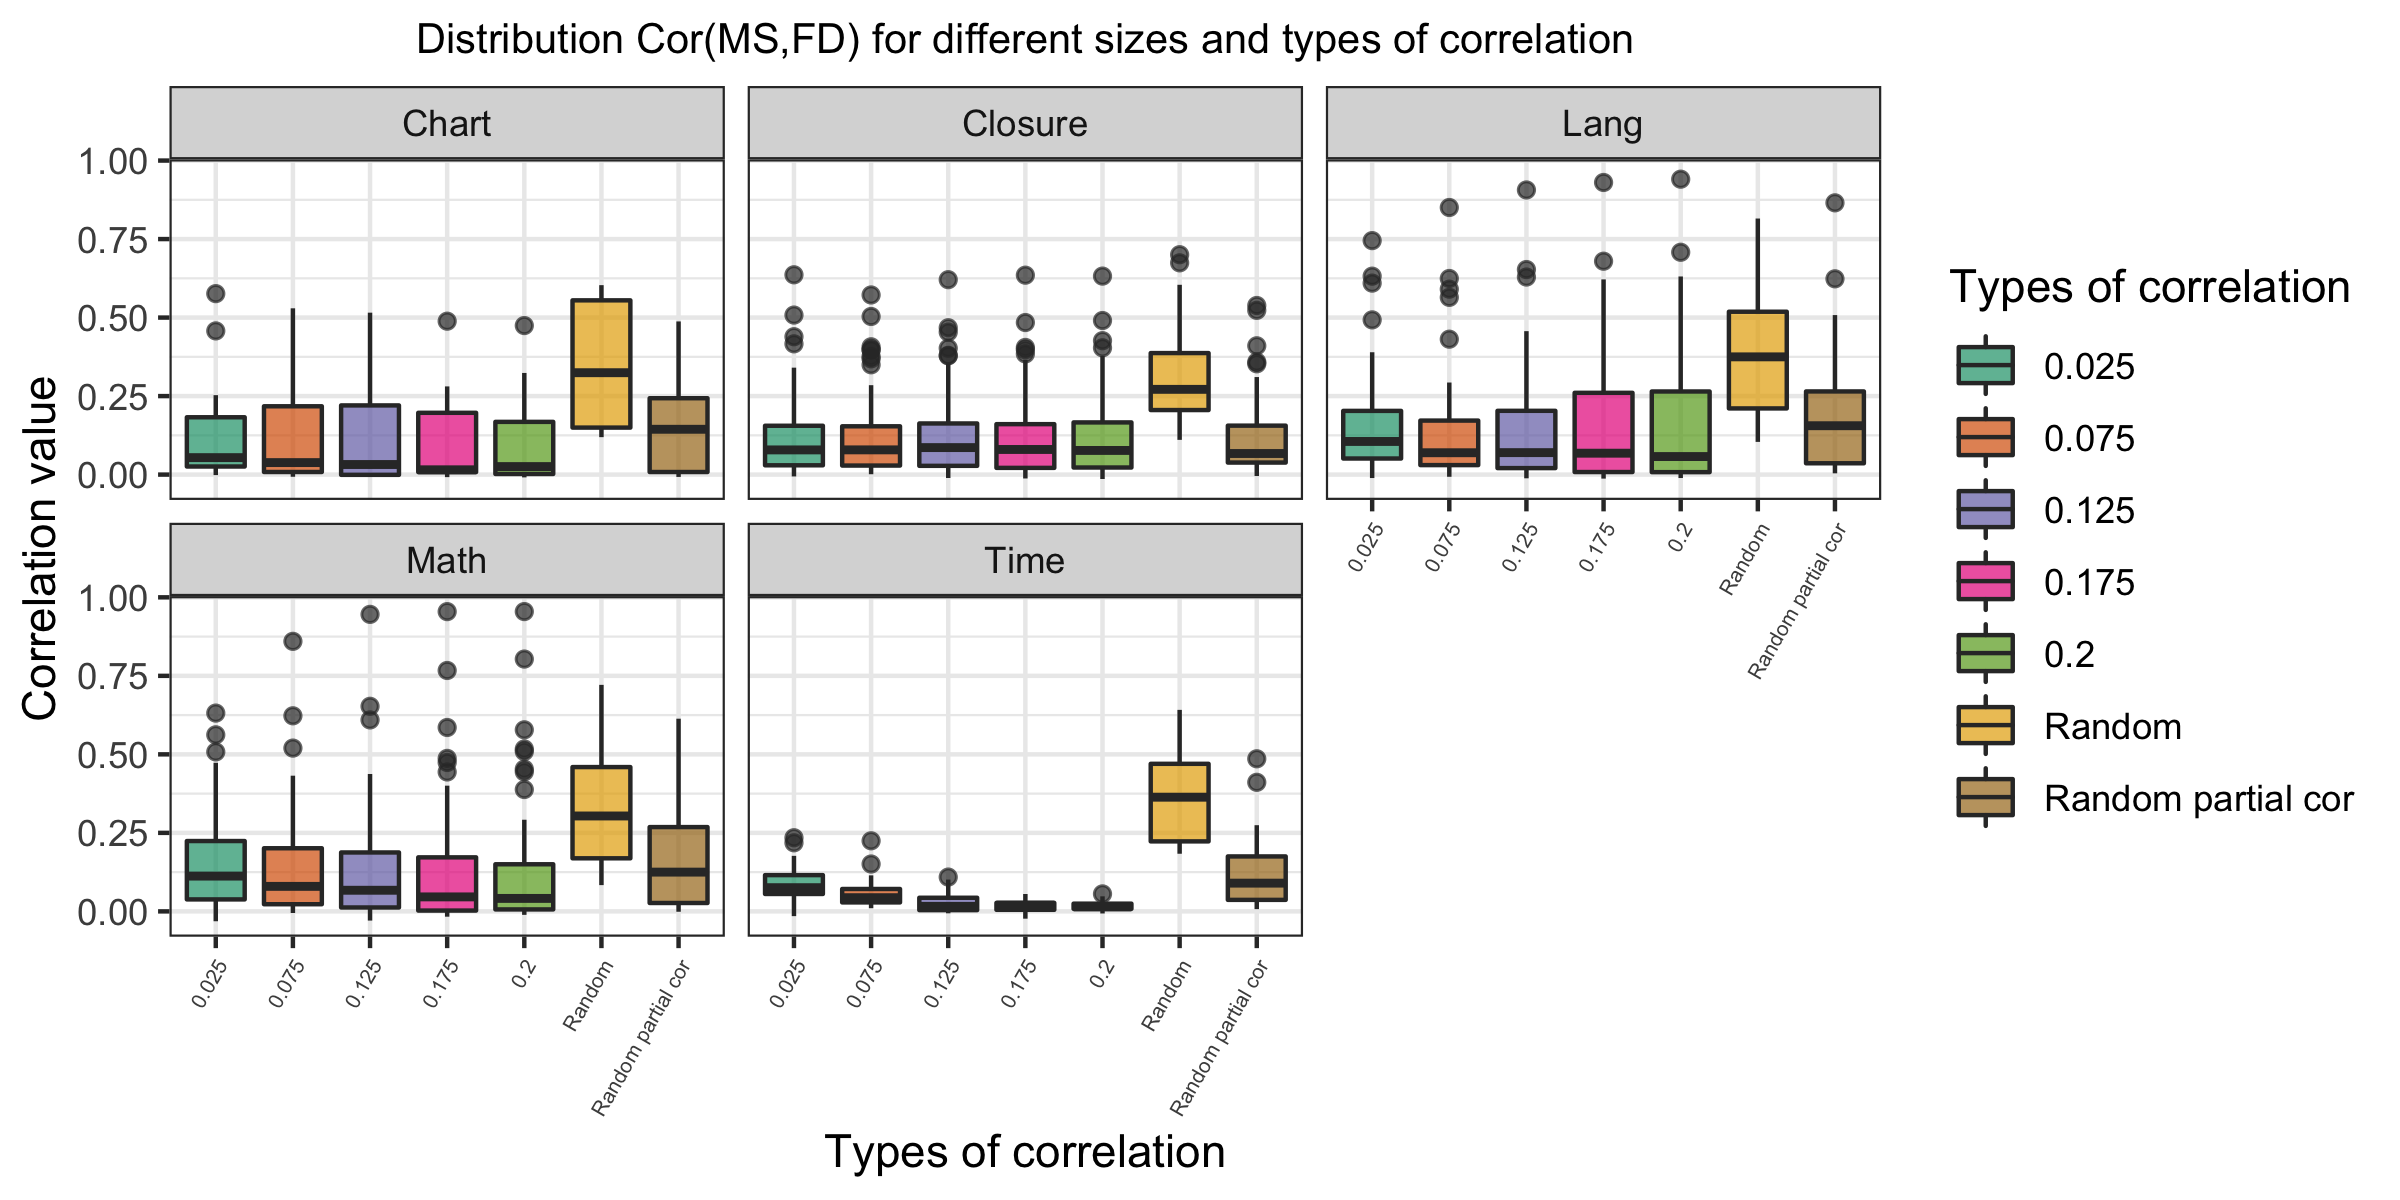
\includegraphics[scale=0.15]{figures/partial_cor_random_fixed.png}
        \caption{Comparing all four (partial) correlations for (mutant score,fault detection) and (test suite size, fault detection) with random and fixed size sampling}
        \label{fig:par_cor_ms_fd}
    \end{figure}


We see from Figure \ref{fig:all_4_cor} that across all projects, partial correlation adjusted for the other variable (MS or size) in general decreases. However, we see that the maginitude of decrease seems to be more pronounced for the correlation between size and fault detection adjusting for mutation score! If anything, one could argue that mutation score is a confounder for the pathway of $size \to FD$. 

In Figure \ref{fig:par_cor_ms_fd}, we only look at the correlation between mutation score and fault detection with different sampling schemes. Note that partial correlation in principle achieves what the fixed size sampling aims to do, except that we are looking at some discretized value of uniform distribution instead of a conitnuous density on $(0,0.2)$. Toward this end, we argue that if one is really interested in using correlation as an effect size measure, which in the next section we will demonstrate a few reasons not to, computing the partial correlation directly would be a preferred alternative.

\subsection{Investigating the behavior of maximal correlation}

\subsubsection{Pearson correlation is bounded}

While it's well-known that a Pearson correlation is bounded between -1 and 1, the same limit does not apply to the correlation of a dichotomous variable and a continuous variable. Specifically, the maximal correlation between a normally distributed random variable $X$ and a Bernoulli random variable $Y$ with success probability $p$ is given by  
\begin{equation}
\rho_{X,Y;\max} = \frac{1}{\sqrt[]{2\pi p (1-p)}} \exp(-\frac{1}{2}z_{1-p}^2)
\end{equation} where $z_{1-p}$ is the $1-p$ quantile of a standard normal distribution. 

Therefore, it is not relevant to refer to a 0.8 Pearson correlation being strong and 0.4 correlation being weak; one need to evaluate the strengthen in view of the upper limit. This statistical fact will be relevant after we introduce the class imbalance problem below: note that if the probability of detecting a fault fails into either extremely high $(\geq 0.99)$ or extremely low $(\leq 0.01)$, the maximal achievable correlation would be bounded by 0.26, which is conventionally considered as a low correlation coefficient.

\subsubsection{Two-stage sampling model}

In this section, we use a two-stage sampling model to characterize the limit of the Monte Carlo simulation used both in method section and in the original paper. Consider the entire test suite $T_f$ for a fault $f$ and a fixed sampling  ratio $r$, the Monte Carlo sampling without replacement really is to approximate the underlying distribution of all ${|T_f|\choose \lceil r\cdot |T_f| \rceil }$ subsets of size  $\lceil r\cdot |T_f| \rceil$. Now for given $r$ and $T_f$, the real fault detection outcome is either 0 or 1, which is a Bernoulli random variable with parameter $p_{r,T_f} = 1- \frac{{|T_f|-|G|\choose \lceil r\cdot |T_f| \rceil }}{{|T_f|\choose \lceil r\cdot |T_f| \rceil }}$ if $|T_f|-|G|\geq r\cdot |T_f|$ and $1$ otherwise.

Note that what we calculated above is the exact distribution of fault triggering, without any Monte Carlo approximation. If we further approximate the distribution of mutation score using a normal, we can compute the maximal correlation for all different Java programs as a function of sampling ratio. We include two programs as a proof of concept analysis in Figure  \ref{fig:maximal_cor_2_program}. Now we can see that Math-6f validates our hypothesis in the last section: when the sampling ratio is above about 5\%, the maximal correlation drops down to negligible values. 

  \begin{figure}[ht!]
        \centering
        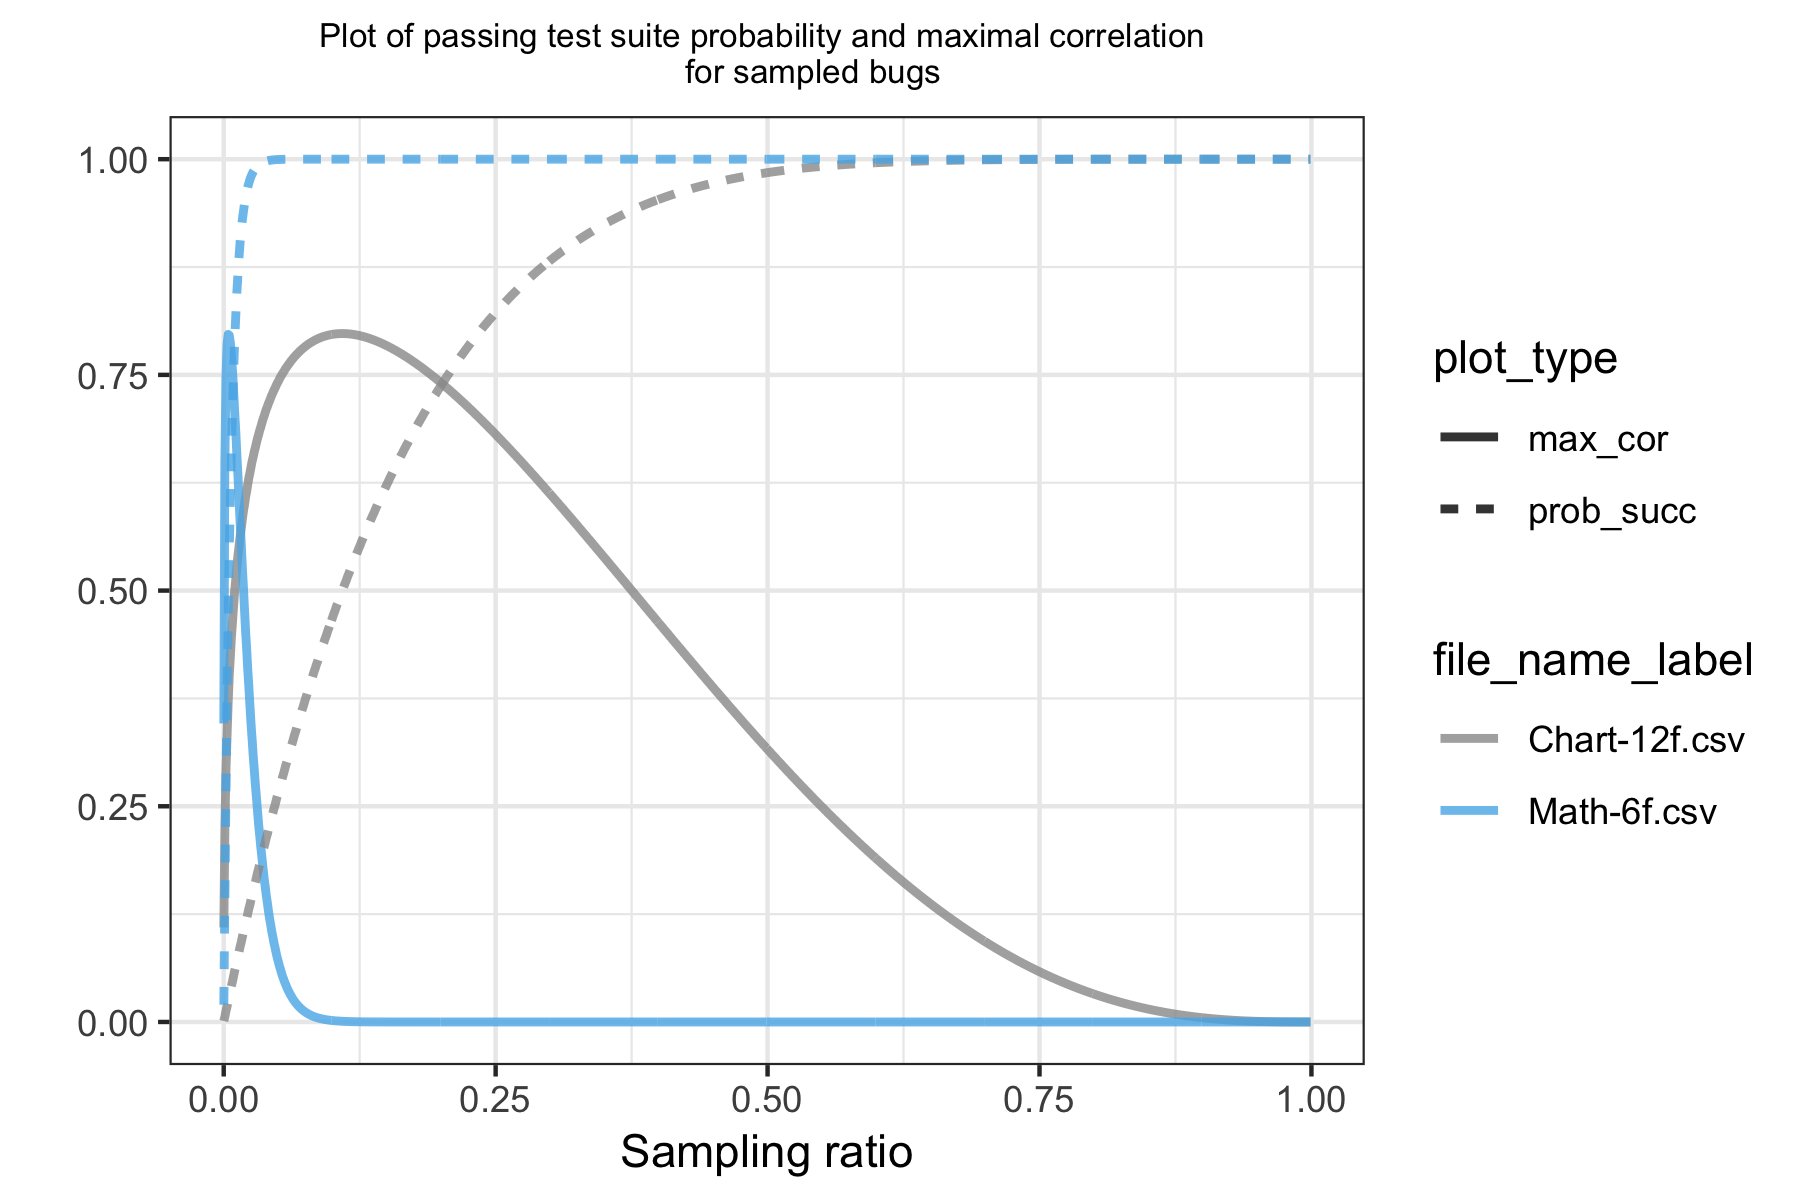
\includegraphics[scale=0.15]{figures/sampled_prob.png}
        \caption{Maximal correlation for two Java programs as a function of sampling ratio}
        \label{fig:maximal_cor_2_program}
    \end{figure}

When we proceed to compute the maximal correlation for all 231 programs (See Figure \ref{fig:max_cor_all_231}), we see that there is a huge heterogeneity in terms of the trend of maximal correlation; therefore aggregating over these sampling ratios and programs within a project might be misleading and not representative of underlying relationship. To sum up, in this section we demonstrate a few overlooked shortcomings of using correlation to characterize the effect size of mutation score onto fault detection. 
    

  \begin{figure}[ht!]
        \centering
        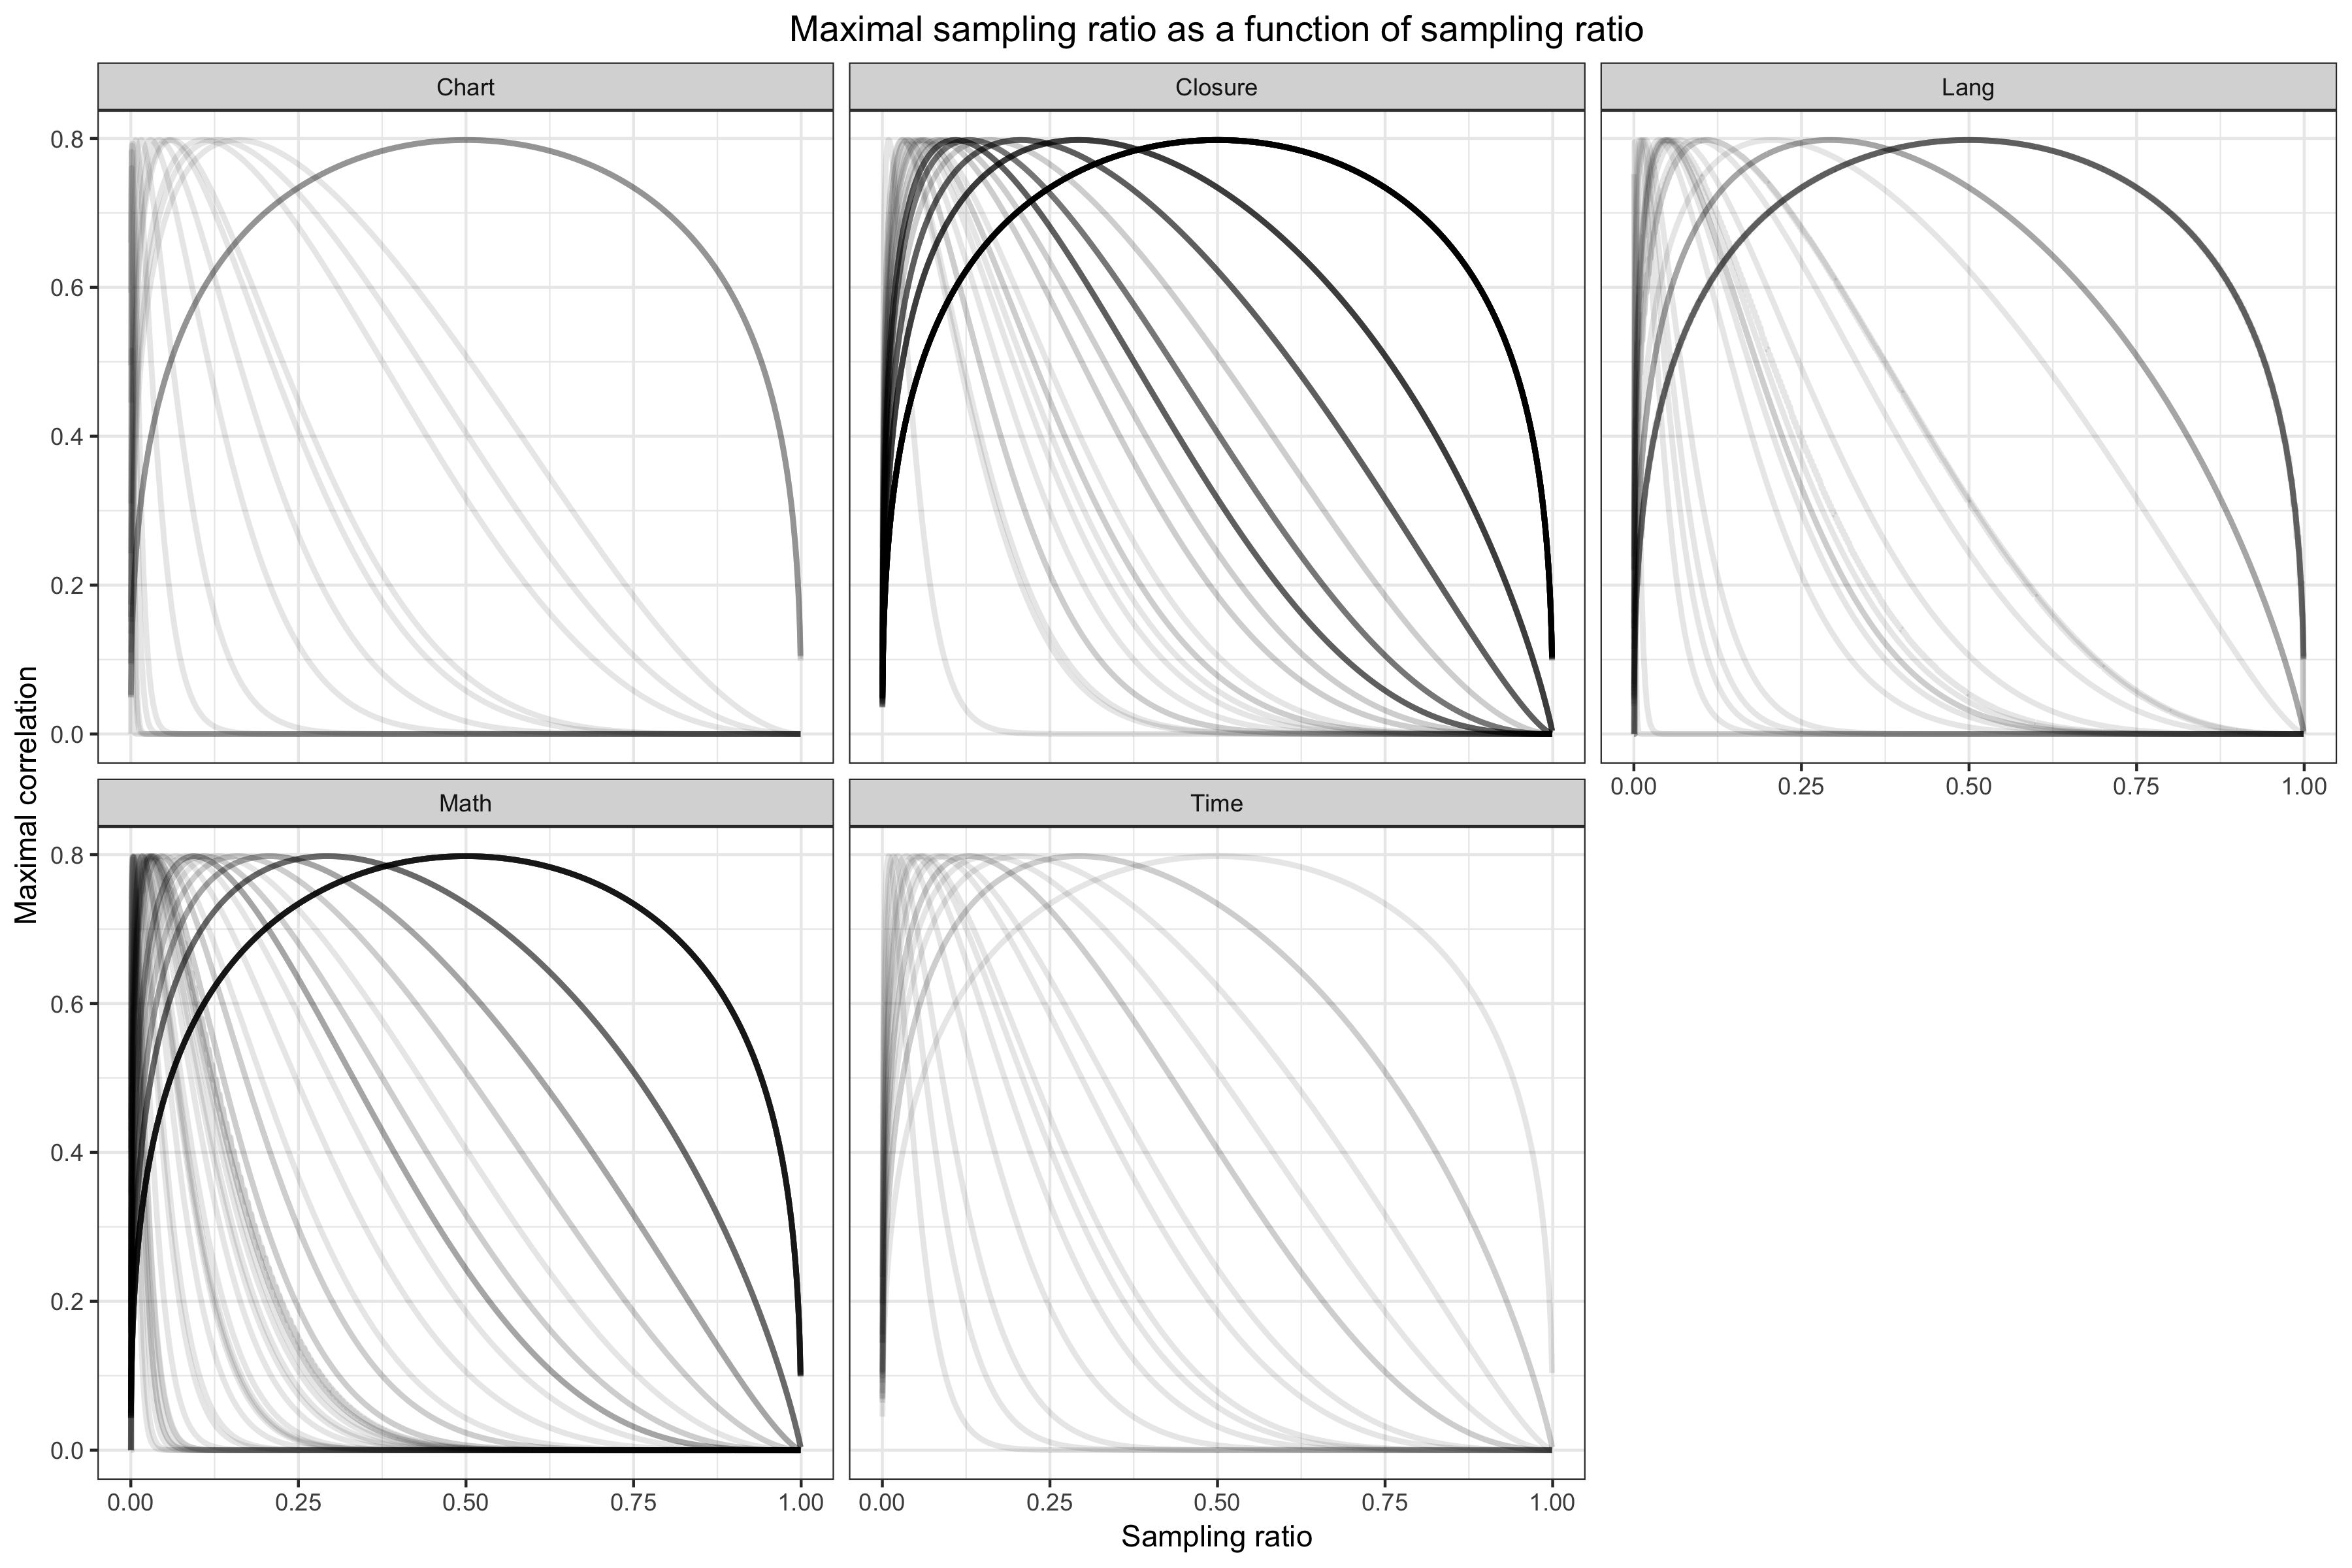
\includegraphics[scale=0.07]{figures/maximal_correlation.png}
        \caption{Maximal correlation for all Java programs as a function of sampling ratio}
        \label{fig:max_cor_all_231}
    \end{figure}
    

\subsection{Linear regression}



  \begin{figure}[ht!]
        \centering
        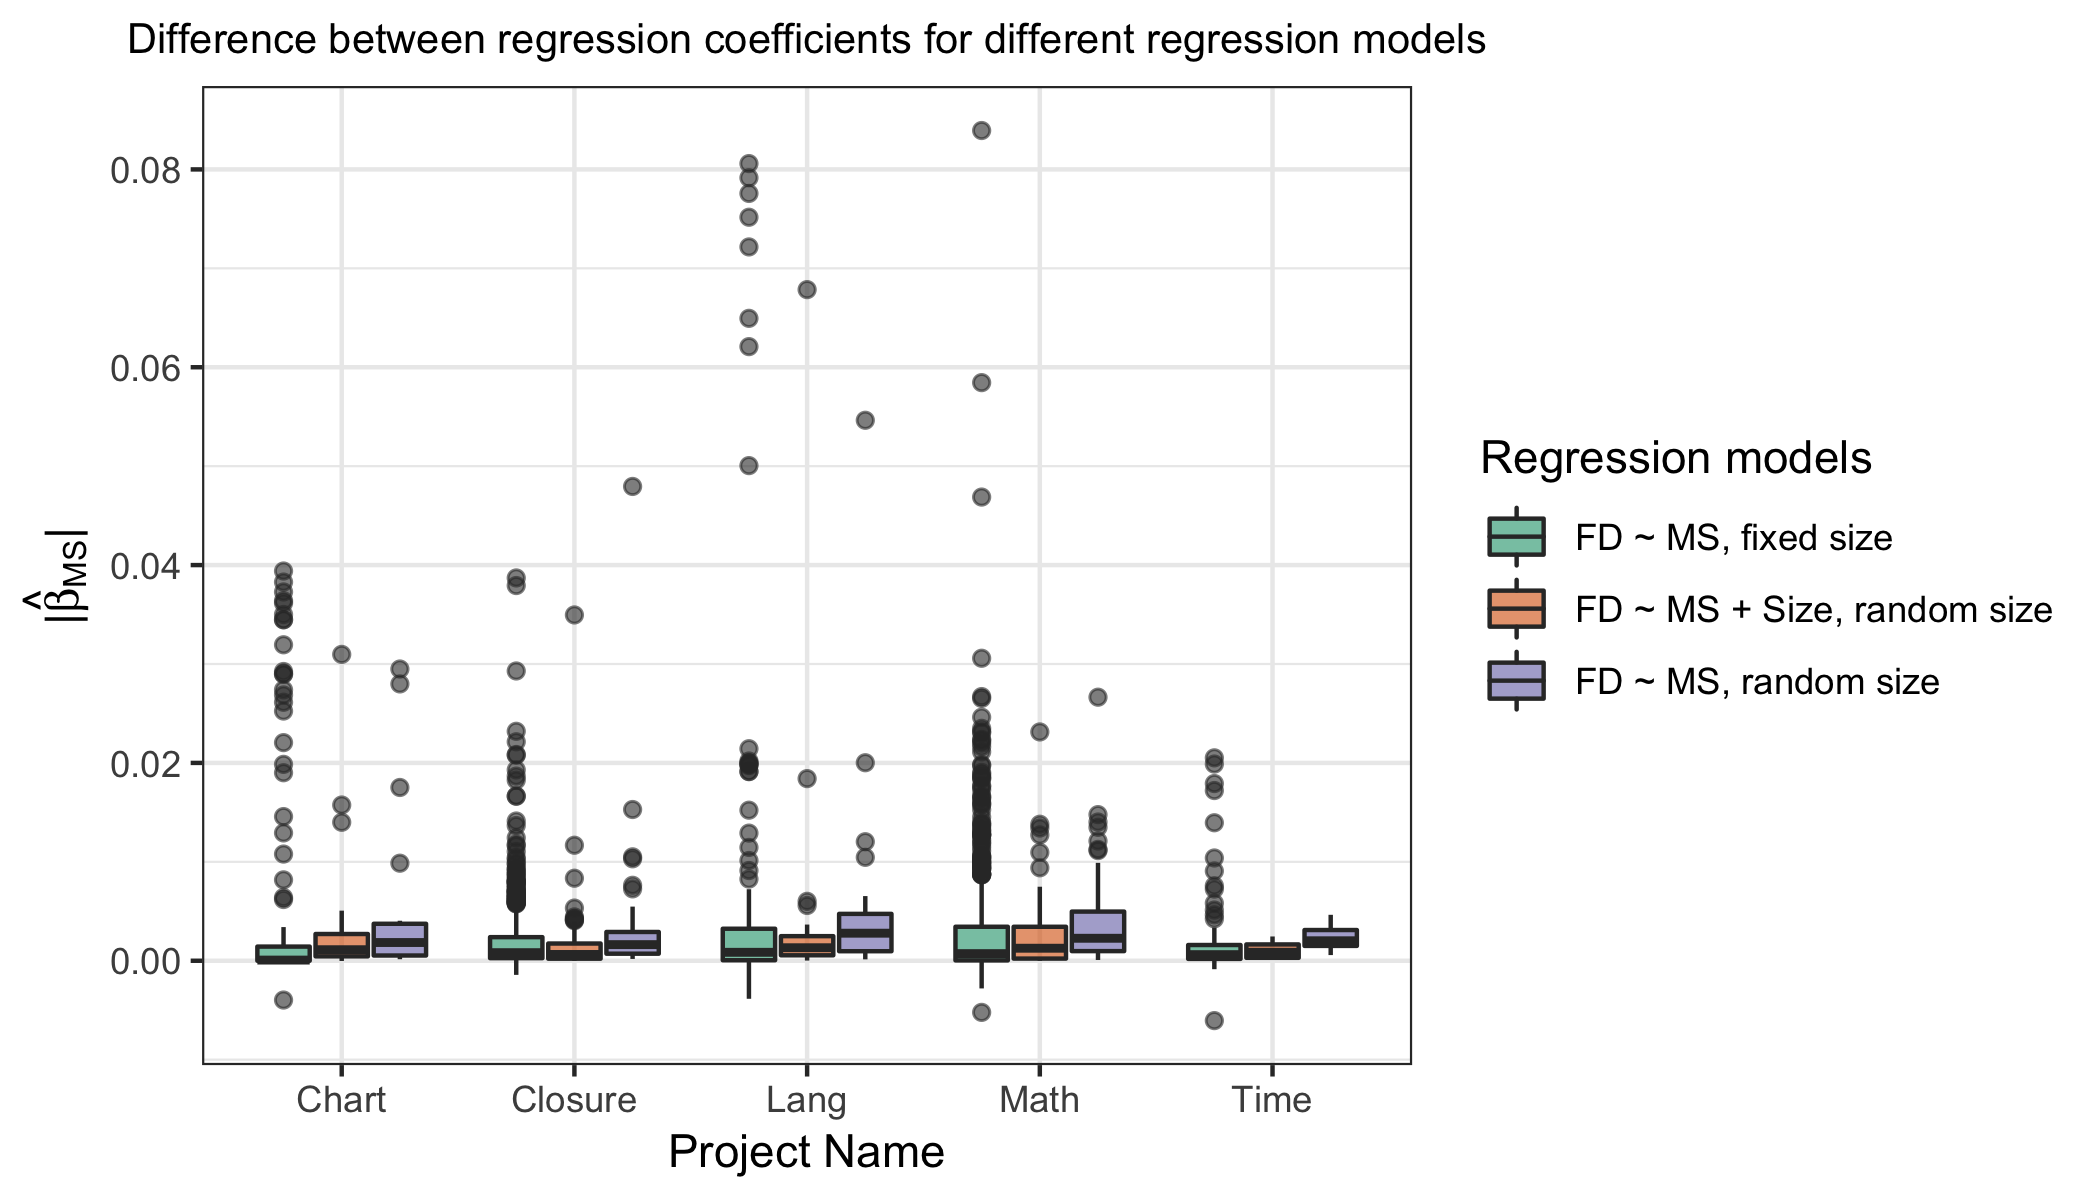
\includegraphics[scale=0.15]{figures/beta_coef_size.png}
        \caption{Estimated regression coefficients for all programs}
        \label{fig:beta_coef_size}
    \end{figure}
    

While linear regression does not guarantee the fitted outcome for a binary variable will stay between 0 and 1, it is a straightforward and valid measure of effect size, if we consider the probability of detecting a real fault is linear in both mutation score and size. We fitted models as described in the method section and compared $\beta_1,\beta^*_1,\tilde{\beta}_1$ (i.e. the effect size of mutation score in three different cases) below (See Figure \ref{fig:beta_coef_size}). We note that when using this alternative effect size measure, the fixed size sampling regression model and random size sampling model adjusting for size give us really similar results. It is not surprising since adding size into the regression equation just implicitly stratifies on size. In addition we see that while not adjusting for size gives us a slightly larger coefficient for mutant score in the random size case, the difference is not nearly as striking as that computed from correlation; further validating the point that correlation alone is an incomprehensive measure of effect size. 

      \begin{figure}[ht!]
        \centering
        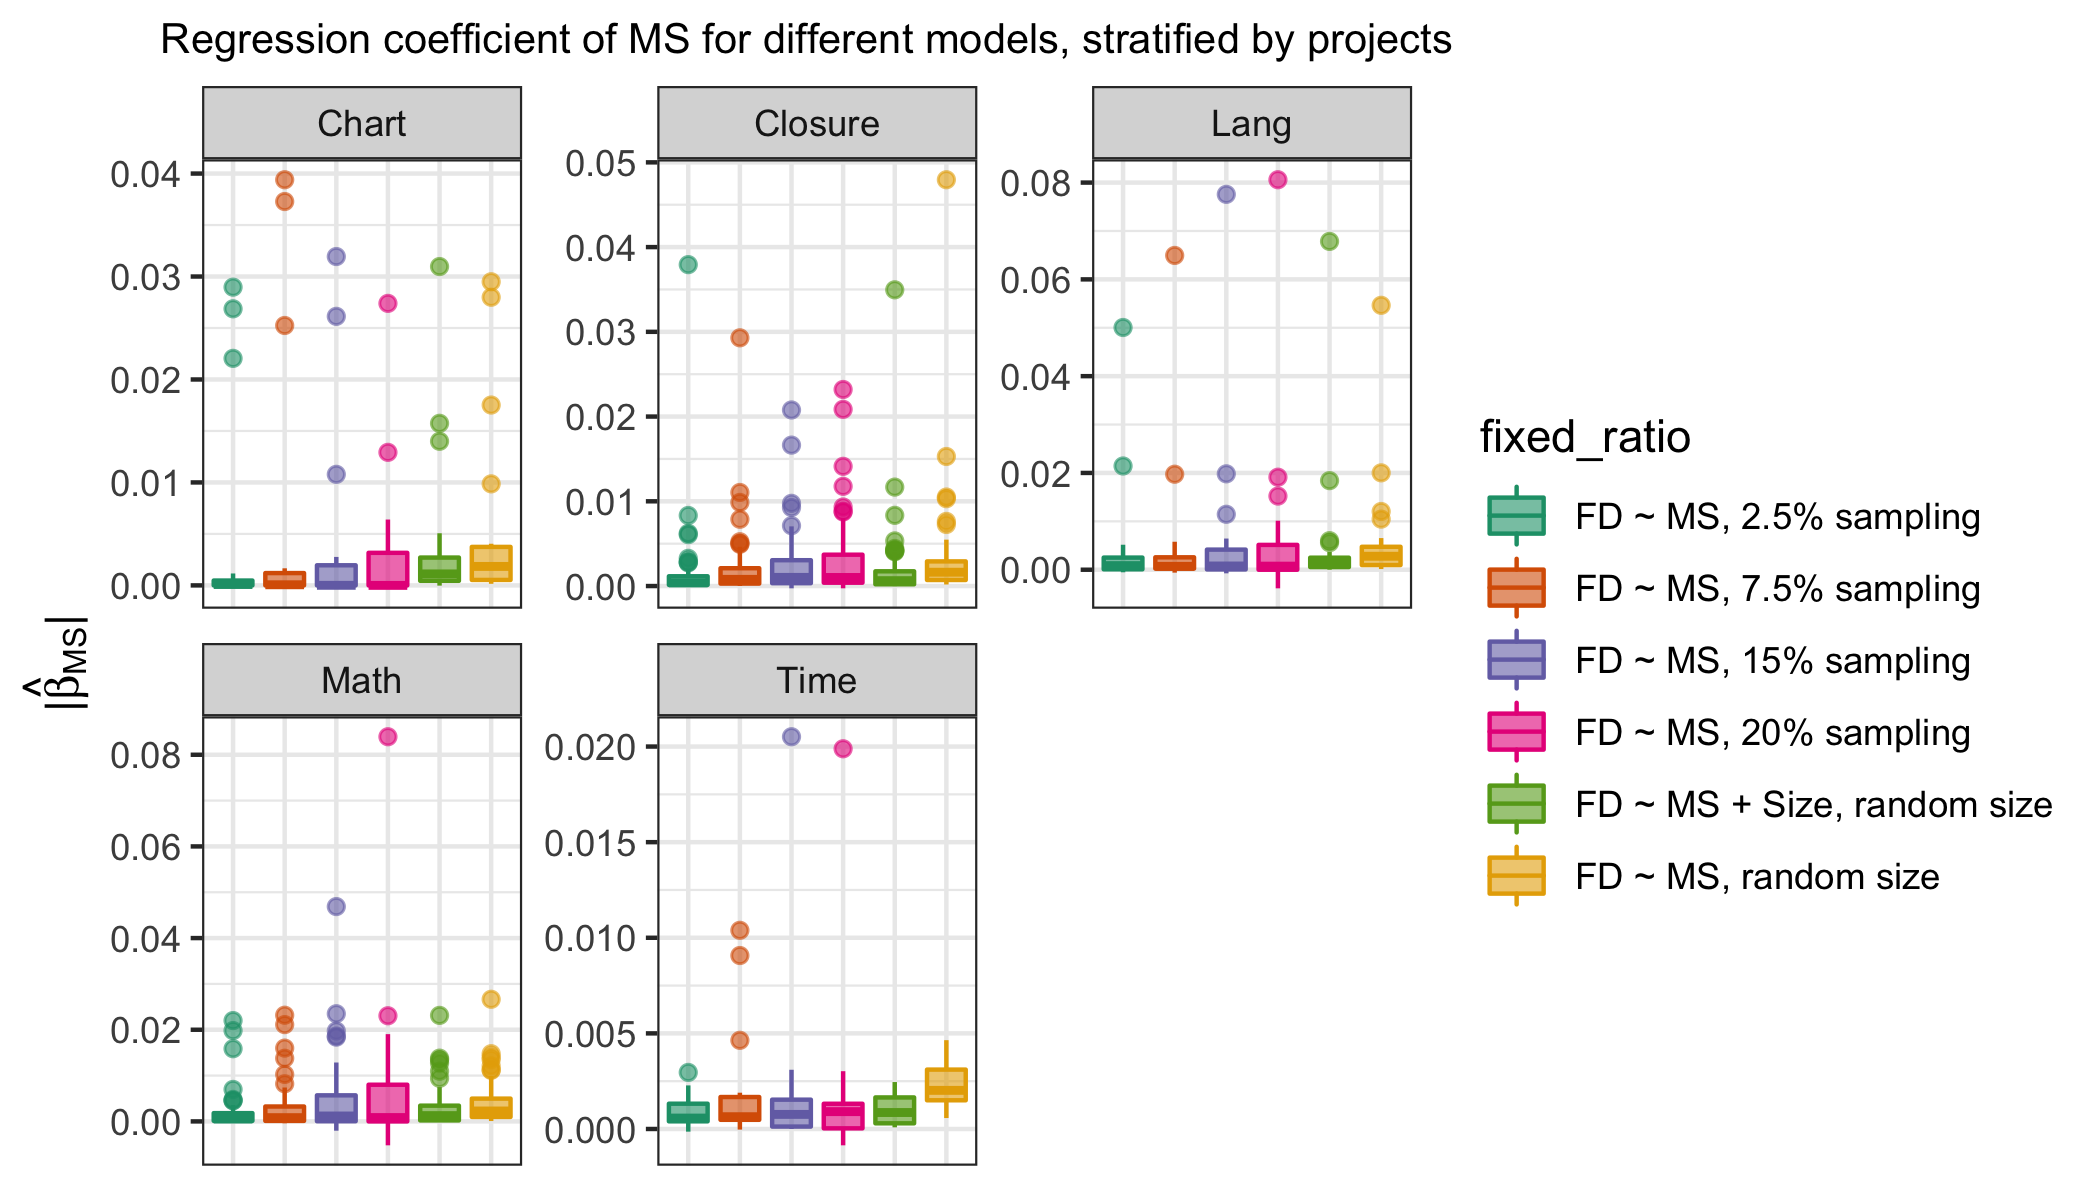
\includegraphics[scale=0.15]{figures/stratified_beta_coef_size.png}
        \caption{Estimated regression coefficients for all models considered}
        \label{fig:stratified_beta_coef_size}
    \end{figure}



We also include Figure \ref{fig:stratified_beta_coef_size} to investigate the difference within fixed sampling scheme, among different sampling ratios. There appears to be no significant difference visually.


\subsection{Logistic regression}

Logistic regression is a far more popular choice for modeling a binary outcome and we include below the analogous results as in the last section, except we are reporting the estimated odds ratio, i.e., the exponential of regression coefficients $\beta$. For some of the datasets due to the imbalance in the outcome (virtually all samples will detect the fault), the \texttt{glm} call in \texttt{R} did not converge and we excluded these in our analyses below.

\begin{figure}[ht!]
        \centering
        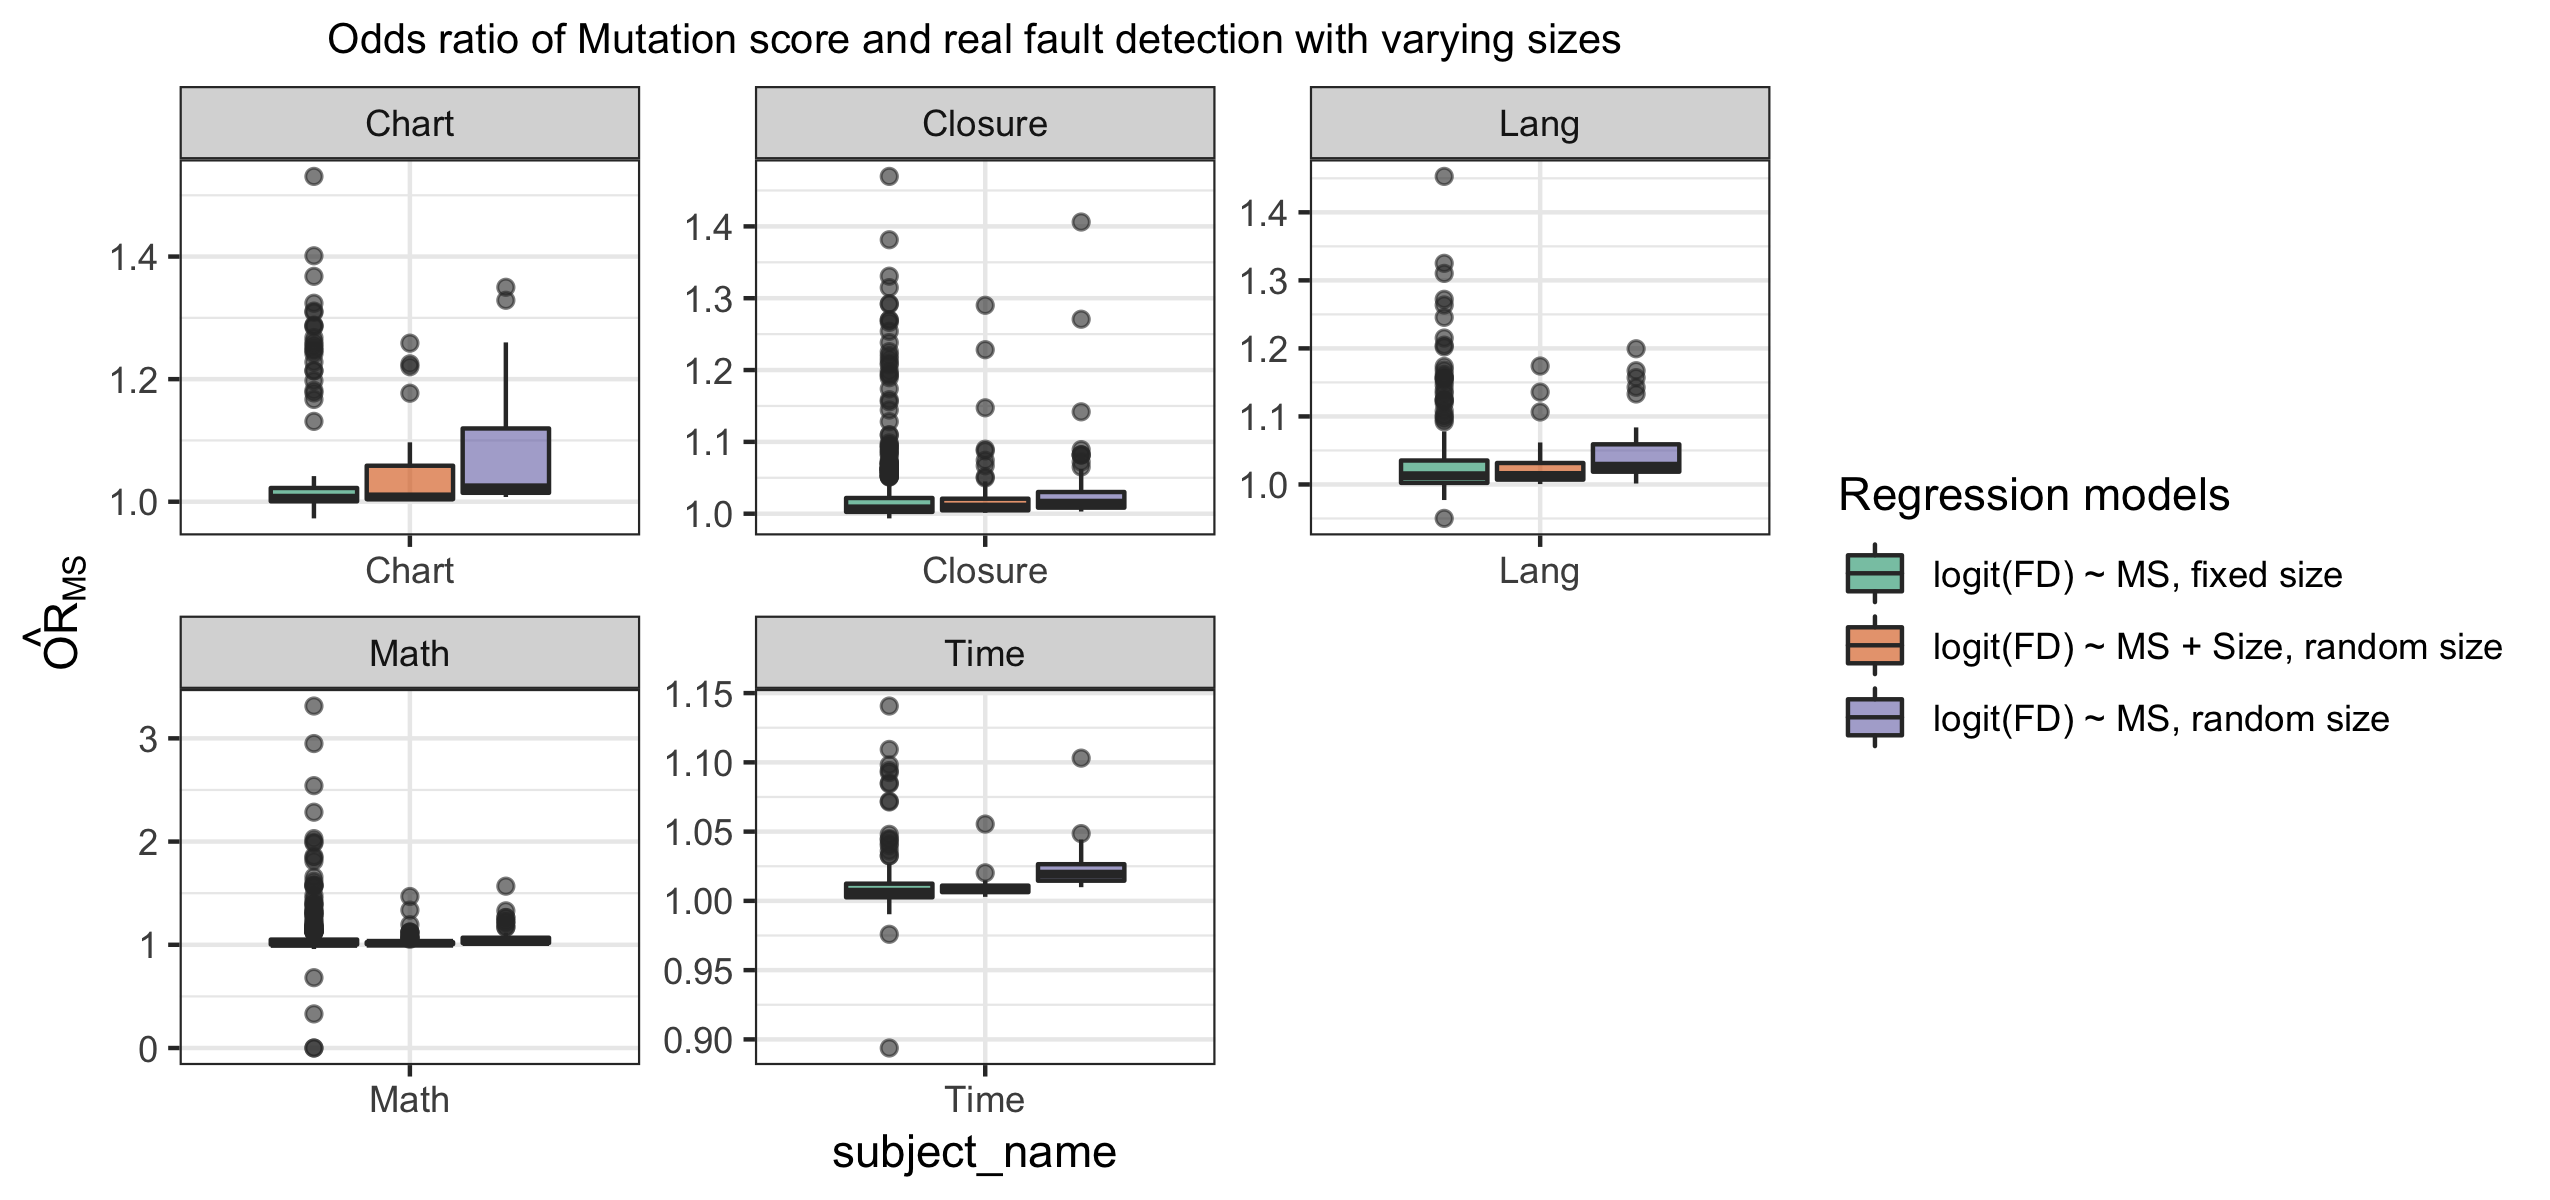
\includegraphics[scale=0.15]{figures/beta_OR_size.png}
        \caption{Estimated odds ratios for all programs}
        \label{fig:beta_OR_size}
    \end{figure}
    
In  Figure \ref{fig:beta_OR_size}, we see a similar trend as in linear regression: adjusted odds ratio is very similar to fixed sampling; both are attenuated compared to the unadjusted odds ratio.

  \begin{figure}[ht!]
        \centering
        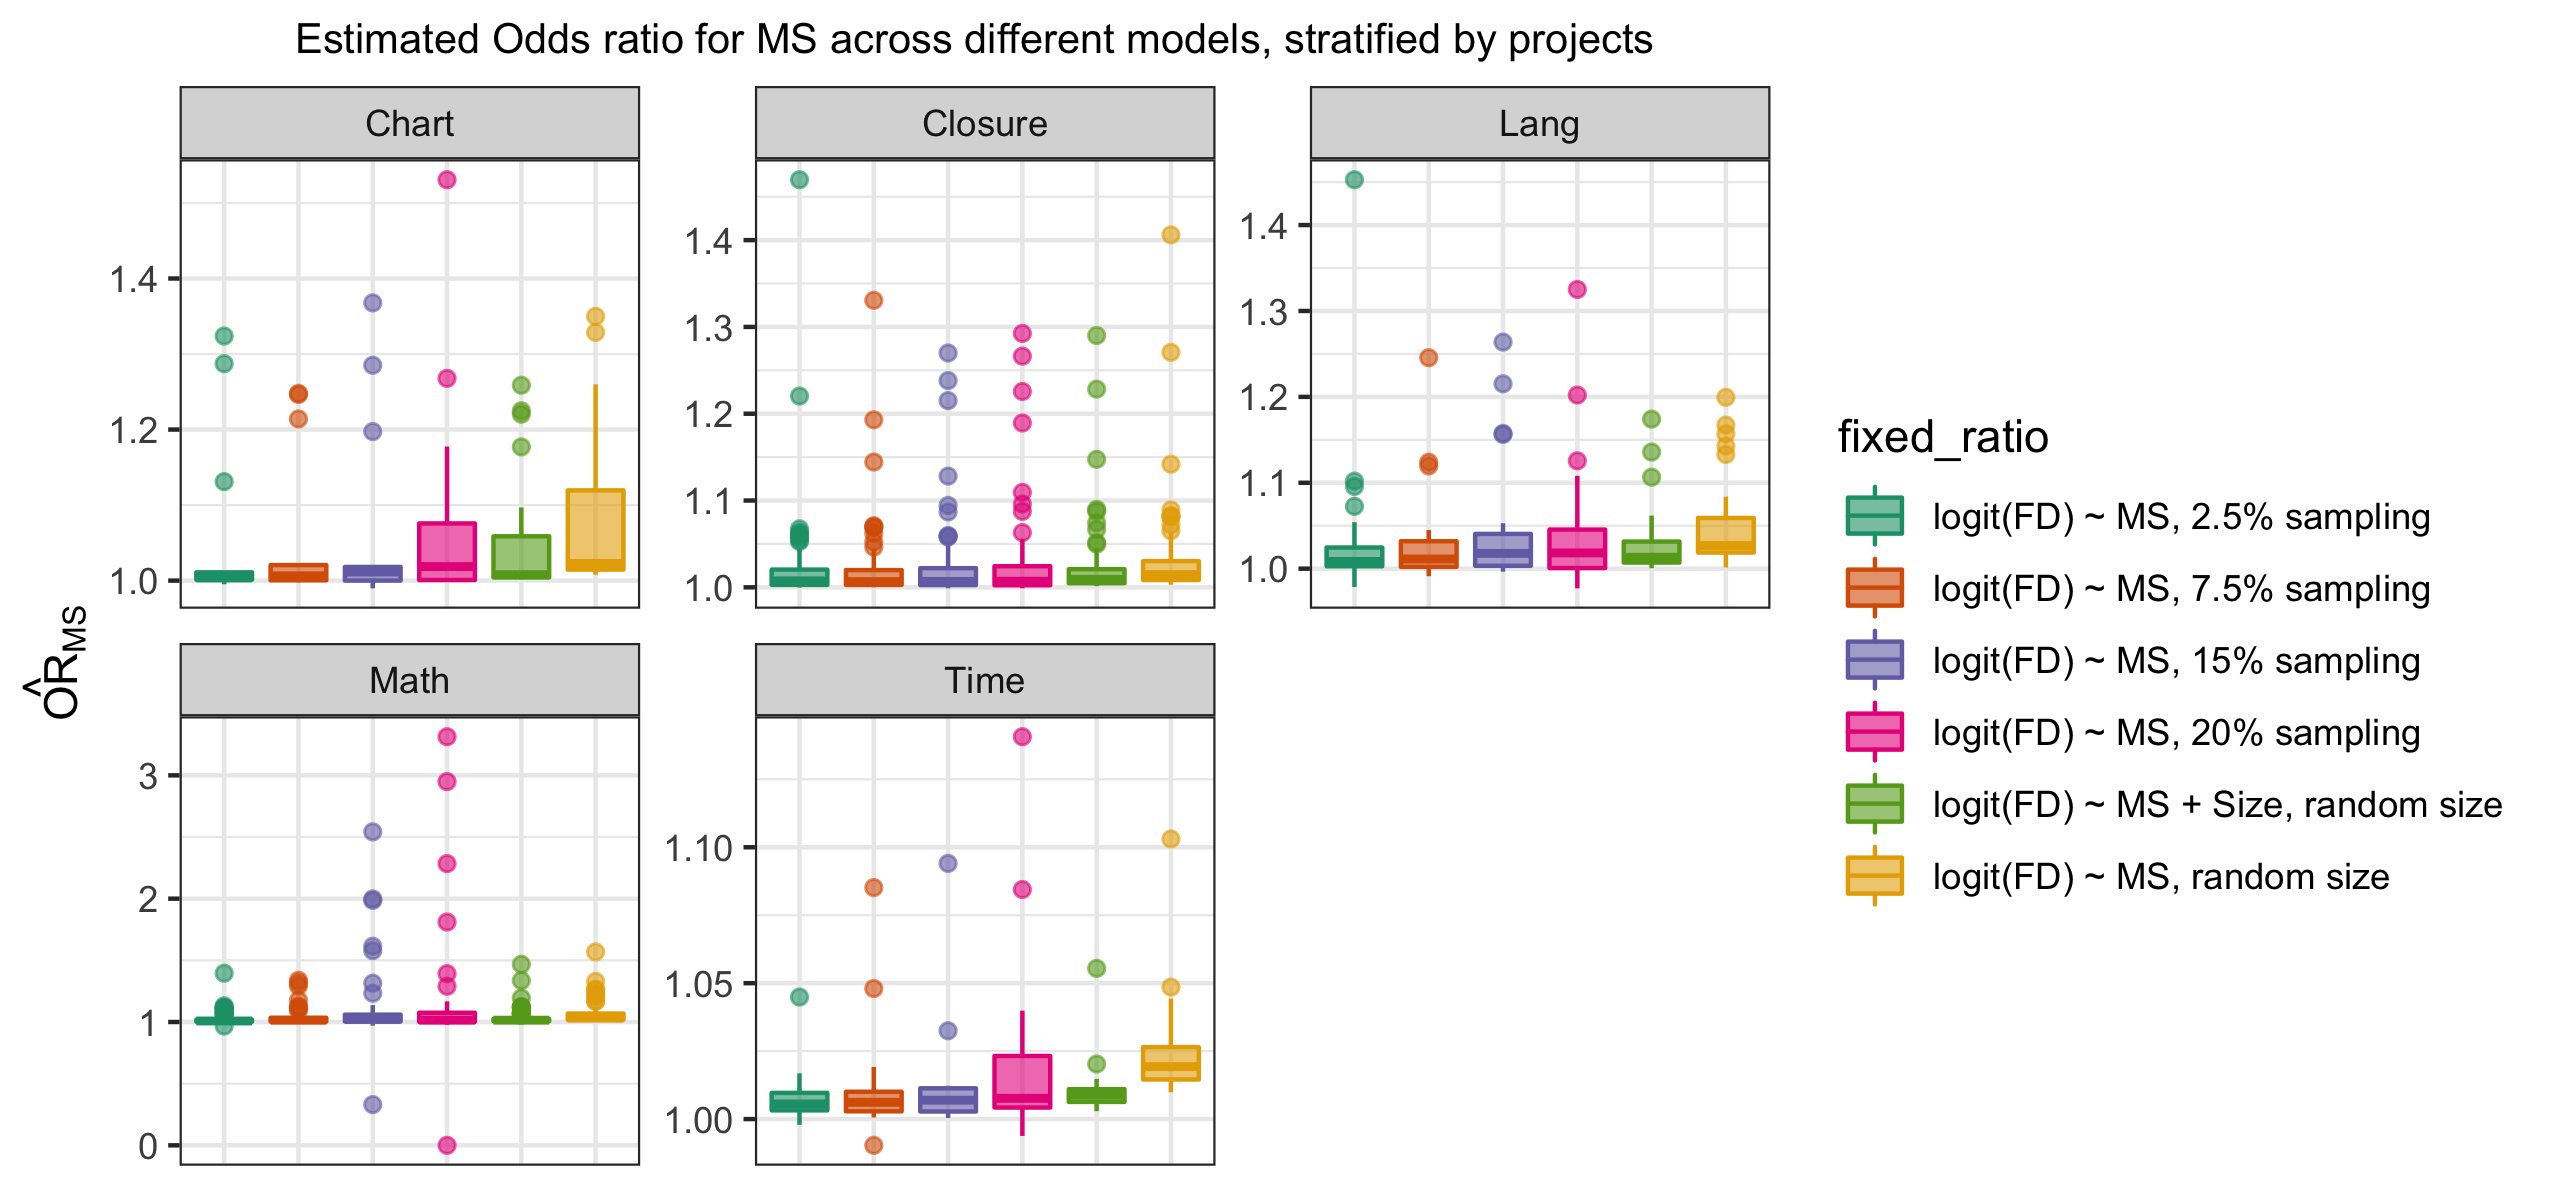
\includegraphics[scale=0.15]{figures/stratified_OR_coef_size.png}
        \caption{Estimated odds ratios for all models considered}
        \label{fig:stratified_OR_coef_size}
    \end{figure}
    


We also include Figure \ref{fig:stratified_OR_coef_size} to investigate the difference within fixed sampling scheme, among different sampling ratios. There appears to be little difference across different sampling ratio visually. Therefore we would recommend using adjusted odds ratio (or other transformations of logistic regression output such as predicted success probablity) instead of manual stratification.

    
\subsection{Coupling}

We now revisit the idea of probabilistic coupling between a mutant and a fault. Recall that coupling is one of the underlying explanations for mutation score based testing: highly coupled mutants lead to more predictive mutation score for real fault detection. For the scope of our project, we looked at the proportion of perfectly coupled mutants across projects and the distribution of coupling probabilities (where perfect couple has probability 1).  

  \begin{figure}[ht!]
        \centering
        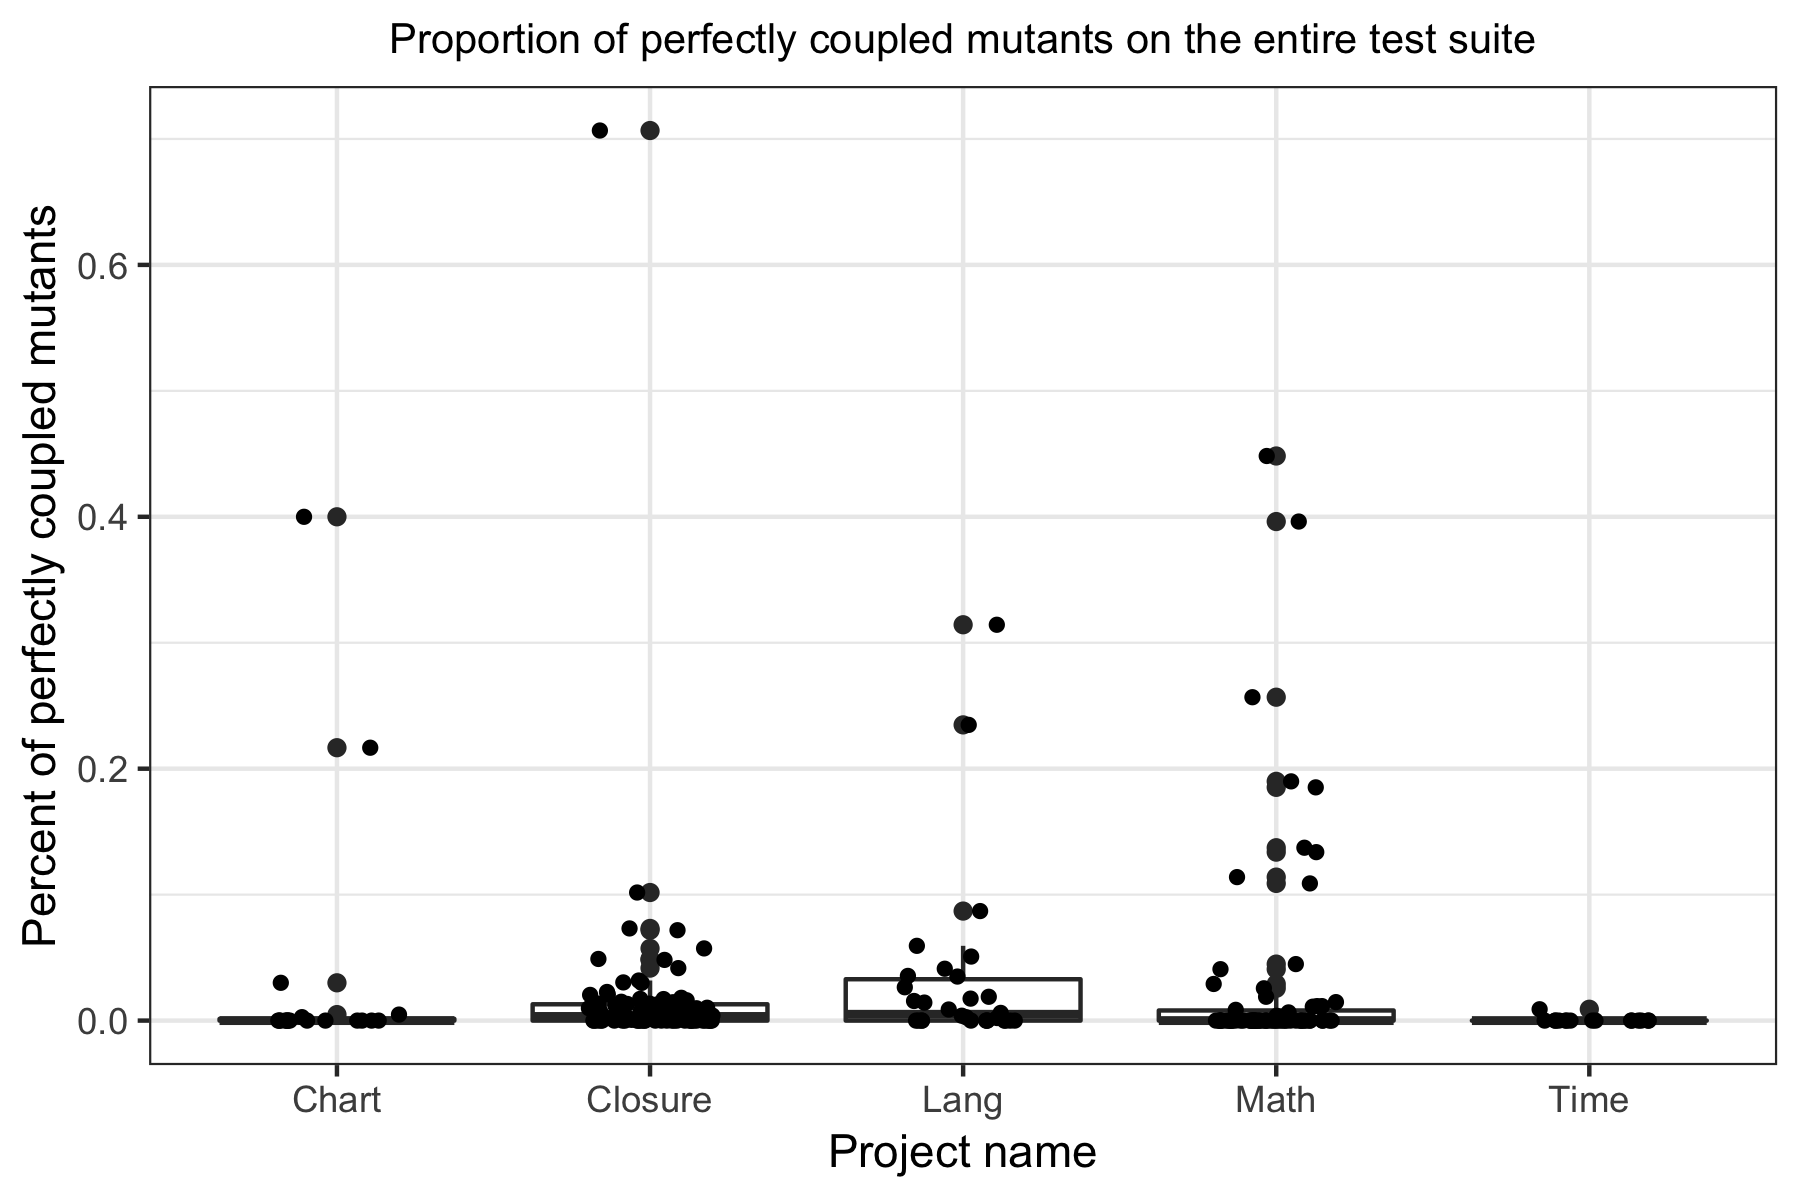
\includegraphics[scale=0.1]{figures/perfect_coupling_prop_box.png}
        \caption{Proportion of perfectly coupled mutants for different tasks, stratified by project }
        \label{fig:perfect_coupling_prop_box}
    \end{figure}
    
      \begin{figure}[ht!]
        \centering
        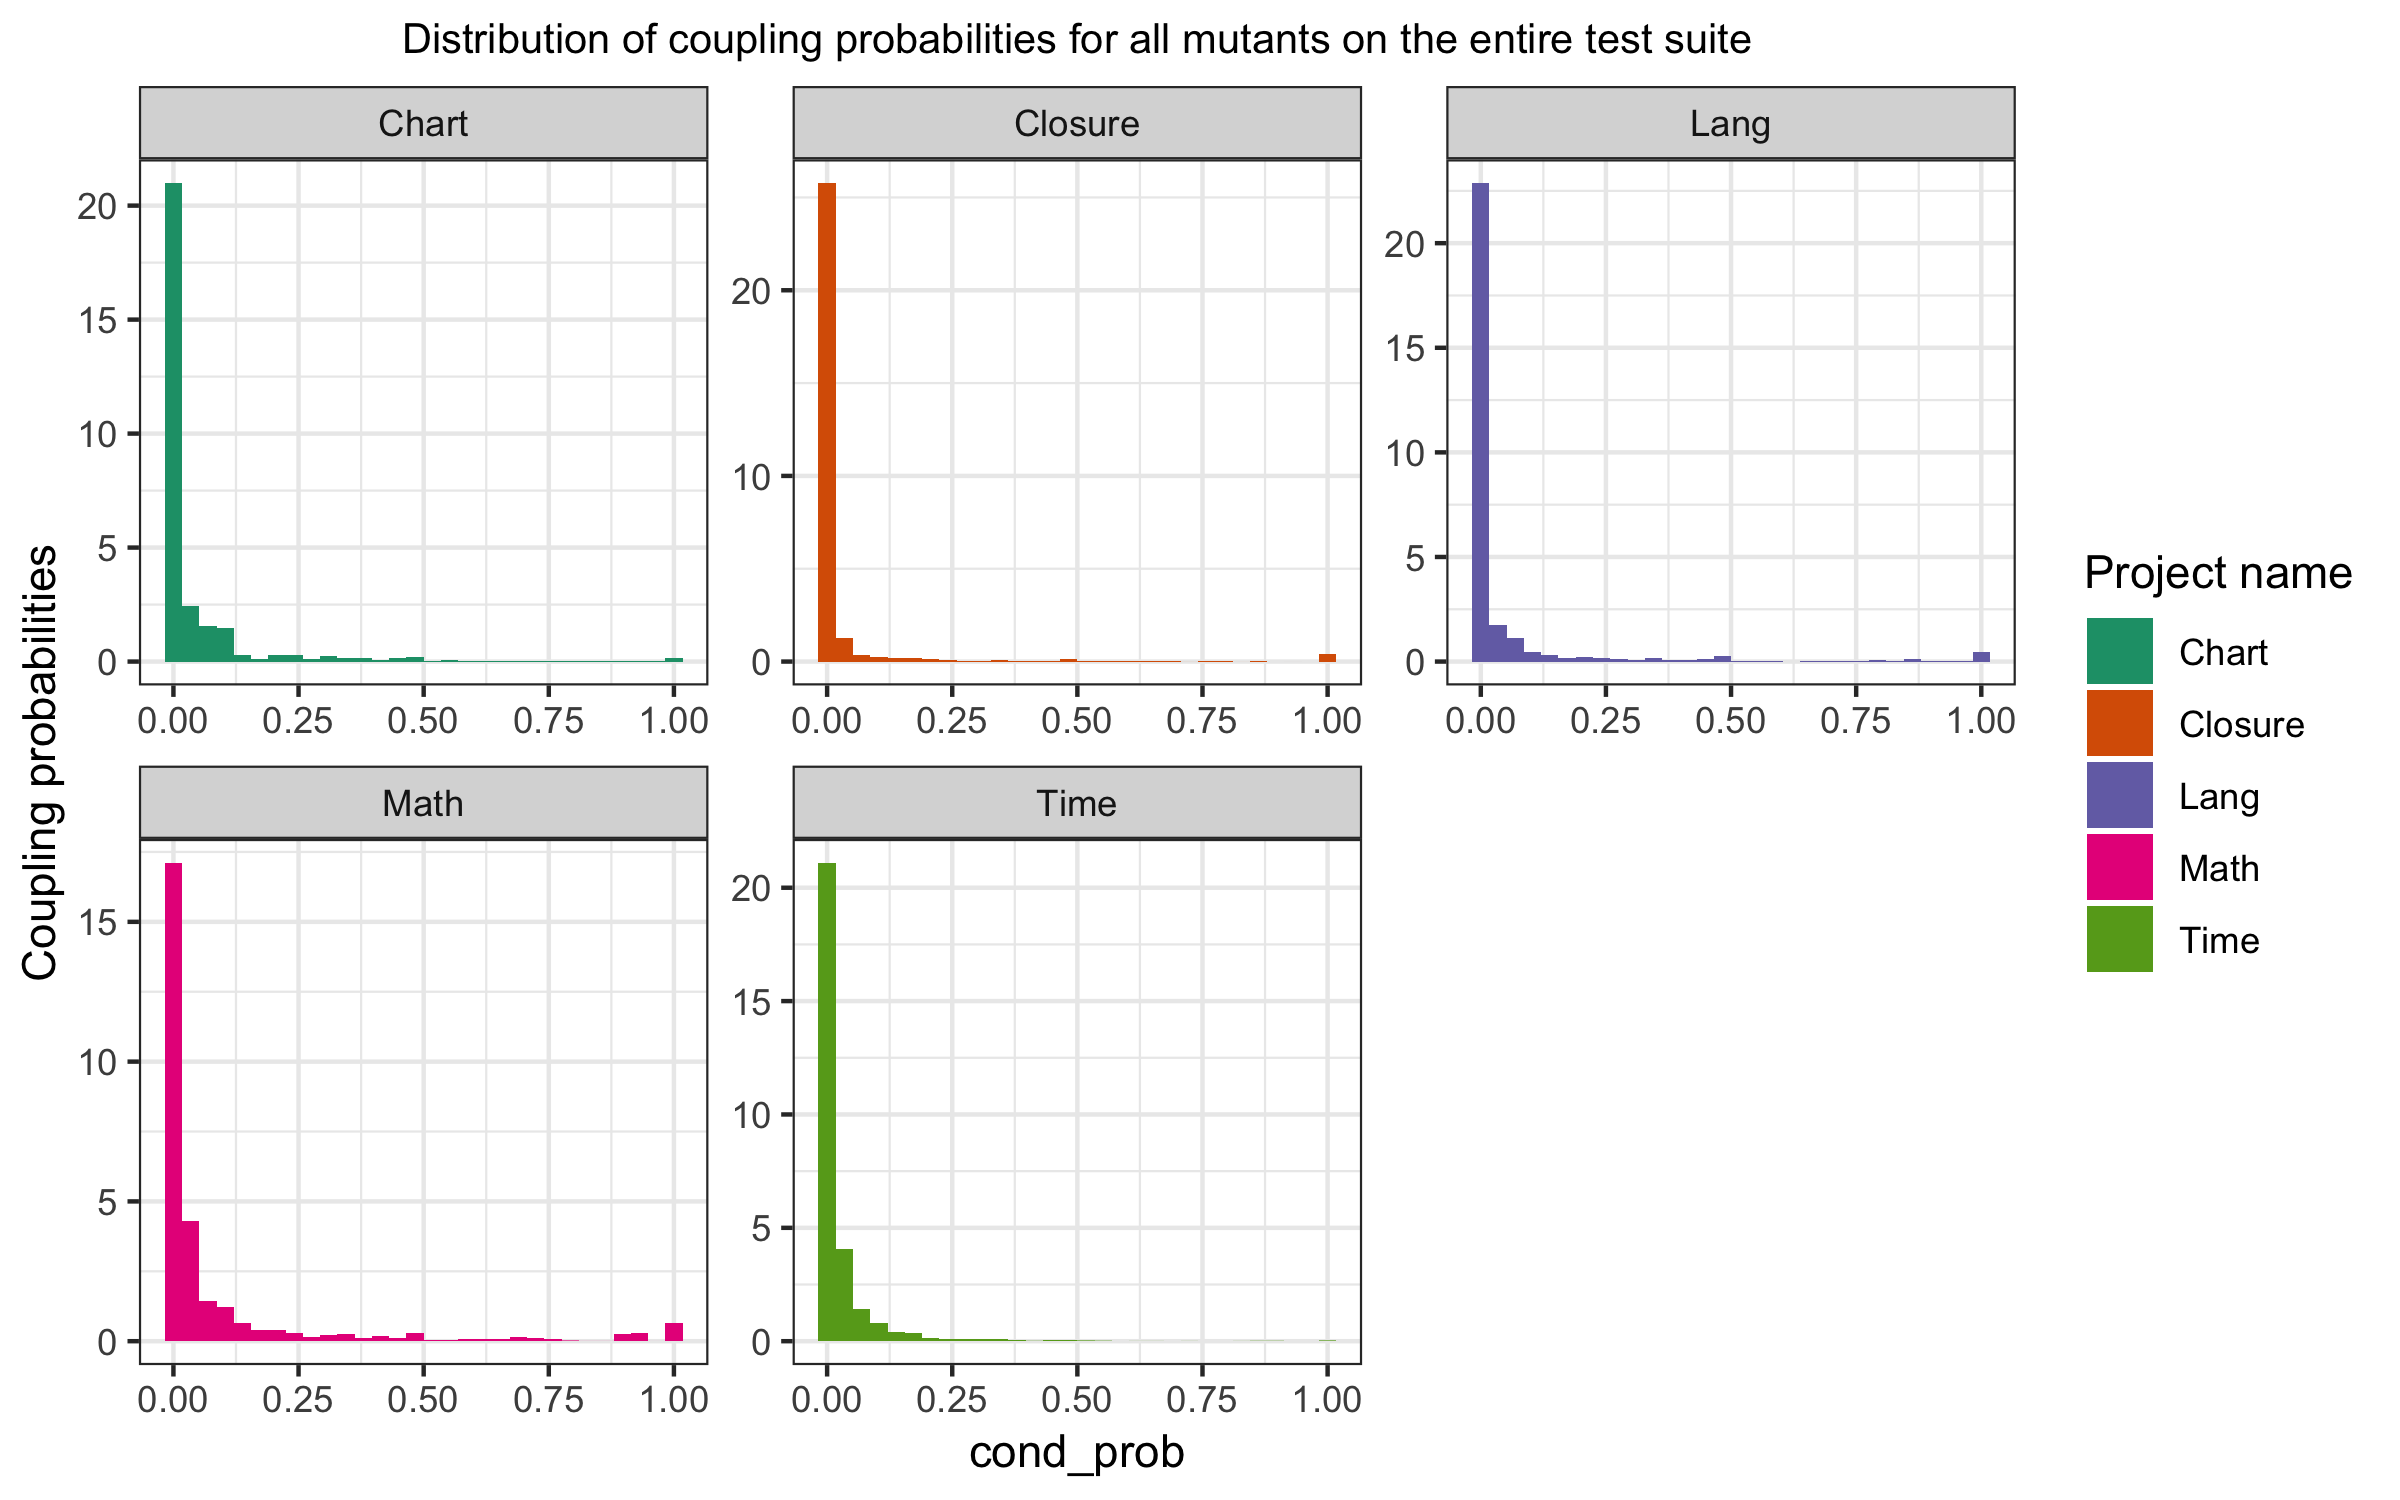
\includegraphics[scale=0.1]{figures/distri_coupling_prop.png}
        \caption{Distribution of coupling probabilities for different tasks, stratified by project}
        \label{fig:distri_coupling_prop}
    \end{figure}

    We see in Figure \ref{fig:perfect_coupling_prop_box} that most of the Java programs have a low proportion of perfectly coupled mutants and there is a decent amount of variation across different projects. The distributions of estimated coupling probability (See Figure \ref{fig:distri_coupling_prop}) are visually similar across different projects: most of the mass is concentrated between 0 and 0.1, with some heavy tails close to 0.9-1 for Math and Lang.


    A natural follow-up question is whether coupling status is associated with some of the effect size measures we mentioned above: one would expect tasks with different coupling probability to have different effect size of mutation score. 


  \begin{figure}[ht!]
        \centering
        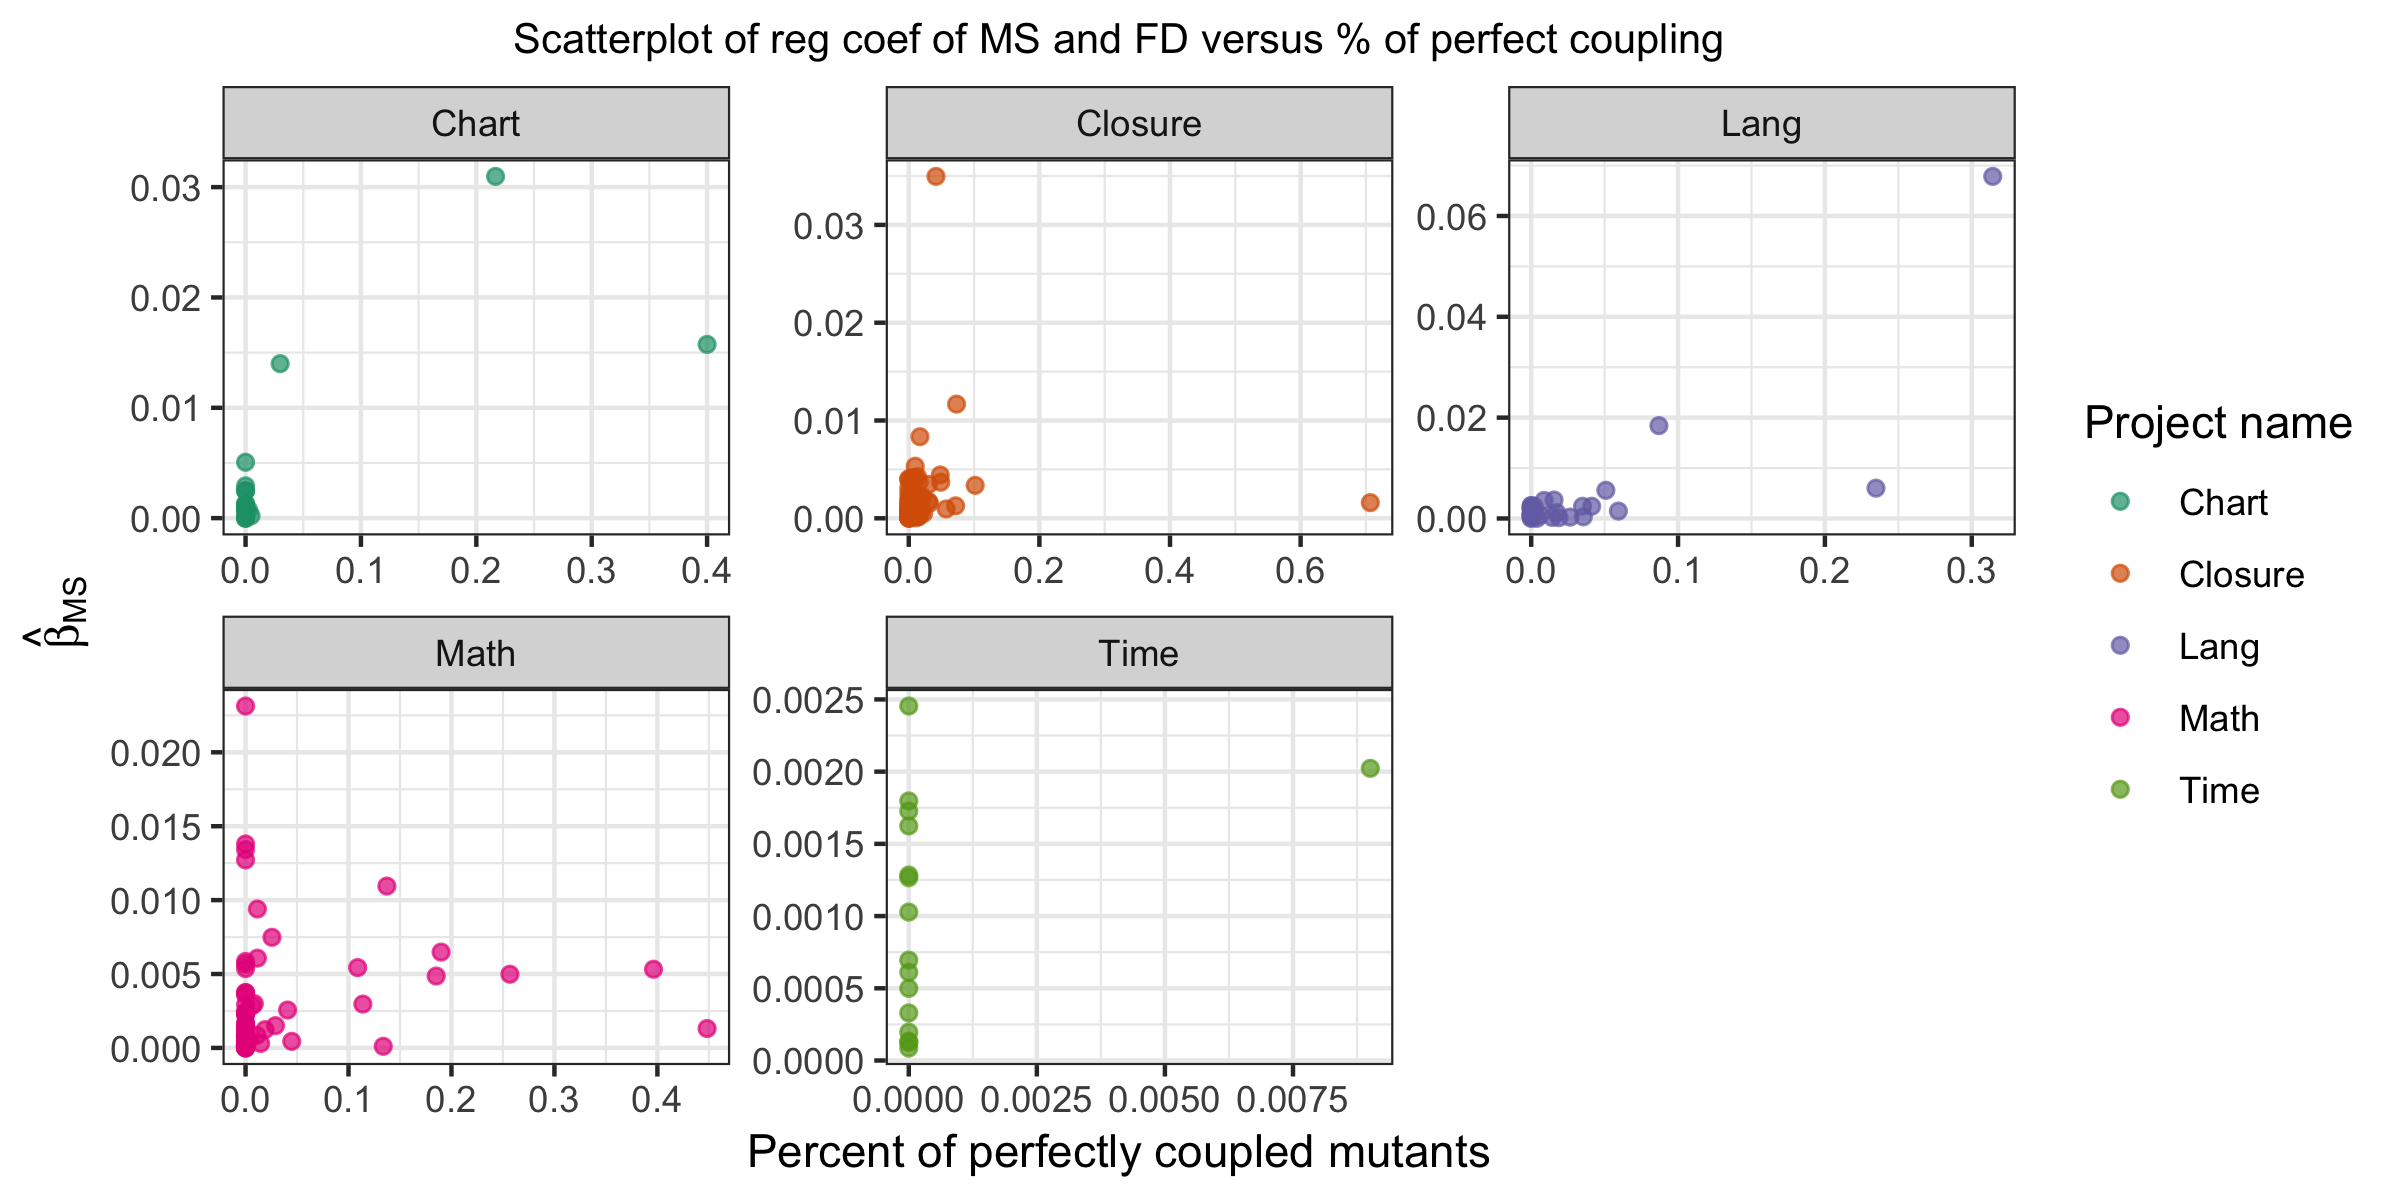
\includegraphics[scale=0.15]{figures/couple_reg_coef.png}
        \caption{Scatter plot of propotion of perfectly coupled mutants and estimated regression coefficient }
        \label{fig:couple_reg_coef}
    \end{figure}

We plotted the estimated regression coefficient $\beta^*_1$ in a size-adjusted model against the proportion of perfectly coupled mutants (See Figure  \ref{fig:couple_reg_coef})  and while we see some trends of positive correlation, more thorough investigation is needed to understand the results. We also included a similar plot for other measures in the appendix. 
    

\section{Discussion}

\subsection{Takeway and recommendations}

Throughout this report we try to answer the one question: is mutation score really correlated with real fault detection? 

We first replicate the results in Papadakis et al. on their Java dataset and explained why the class imbalance problem (from the two-stage sampling model), combined with the boundedness, makes Pearson corrleation a less desriable effect size measure. Moreover, empirically we demonstrated that even if c computing the correlation (with or without controlling for size) is the goal of the study, one could simply use partial correlation to adjust for sizes; instead of reinventing the wheel for Monte-Carlo sampling.

Then the paper shifts its focus onto two alternative effect size measures: linear regression and odds ratio and we see much less change in terms of adjusting for size or not. In addition, we make the same recommend for controlling for variables: instead of stratifying on size manually, one could simply use a regression model with size as a variable on the right hand side. 

Finally we briefly touched on the coupling effect and show that there might be a connection between highly coupled mutants and larger effect size of mutation scores; however this particular path needs more investigation.


\subsection{Threats to validity}

While this paper intends to be an extension and refutation study, we still see a few threats to validity: 
\begin{itemize}
\item
External validity: we did not communicate with the authors on the exact details of their study and therefore our results might not be exactly comparable.

\item

Internal validity: the actual fault detection probability could depend on omitted variables in our study such as the type of test generation mechanism.

\item

Statistical validity: we did not attempt to quantify the difference between adjusted and unadjusted effect size measure and ideally putting confidence intervals on these measures would strengthen our results. In addition most of our discussion on coupling is either theoretical or exploratory data analysis based and therefore lacks statistical ground when one attempts to draw any conclusion from them. 
\end{itemize}

\subsection{Future directions}

As mentioned above, we would like to pursue the direction of the coupling effects further; it would be beneficial both for this study and for the future ones in the community to understand how probabilistic coupling affects effect size measures such as correlation and regression coefficient.

Furthermore, it would also be statistically more sound to include uncertainty quantifications of our effect size measures.


\section*{Supplementary Information}


\subsection*{Miscellaneous}

\begin{itemize}
\item 
Github repo for the study:\url{https://github.com/yiqunchen/correlation_analysis_ms_fd_size}
\end{itemize}


\subsection*{Supplementary figures}


  \begin{figure}[ht!]
        \centering
        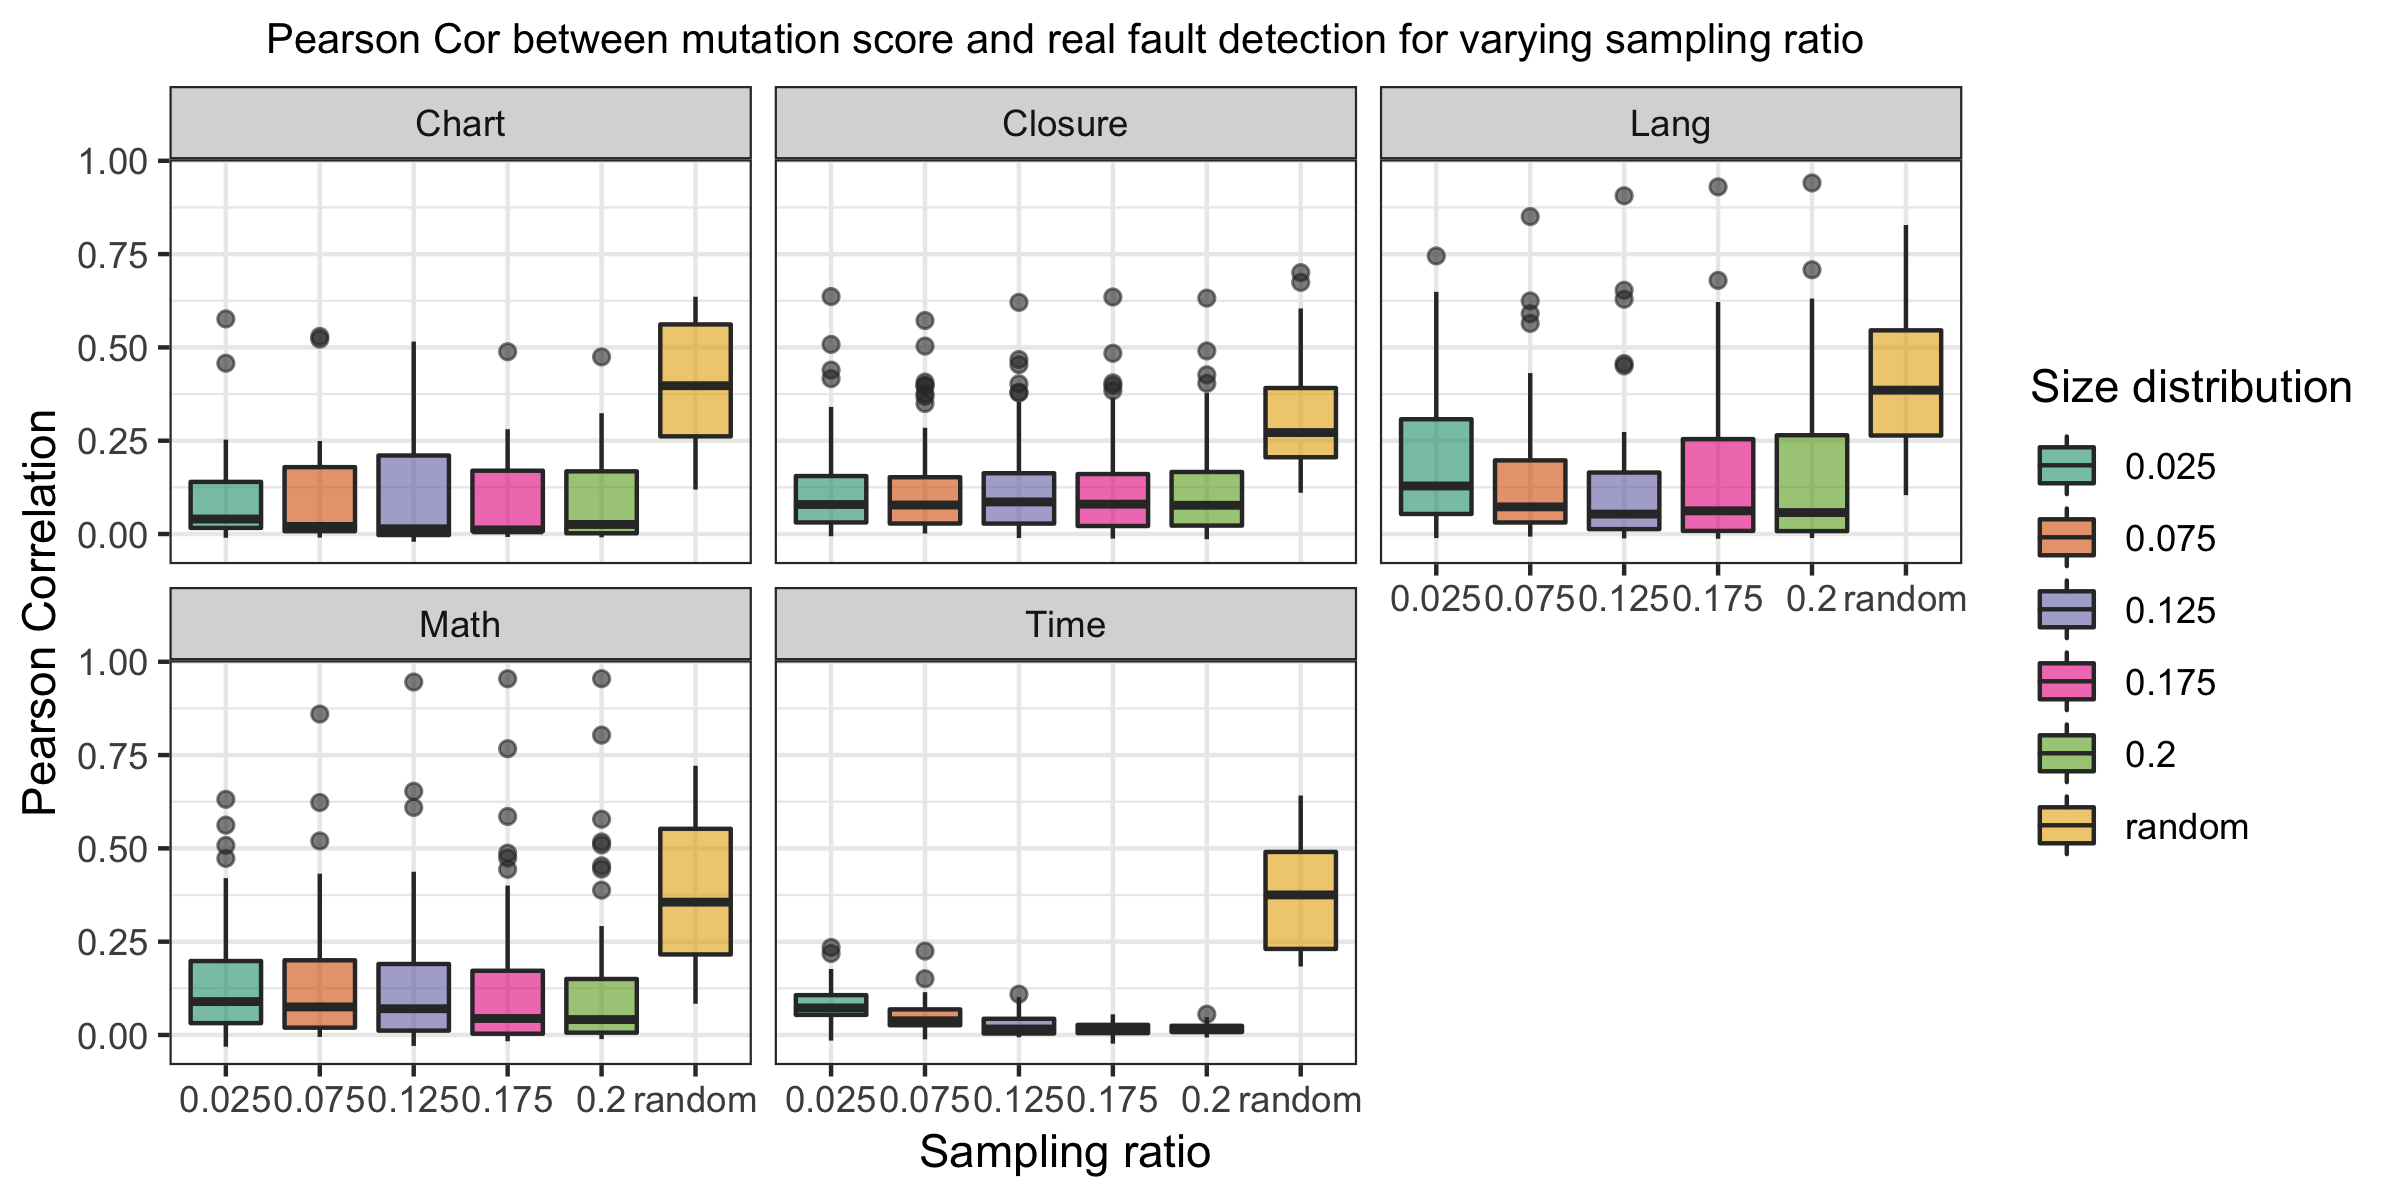
\includegraphics[scale=0.15]{figures/reproduce_fig_3_stratify_size.png}
        \caption{comparing correlations for (mutant score,fault detection) with random and fixed size sampling}
    \end{figure}




  \begin{figure}[ht!]
        \centering
        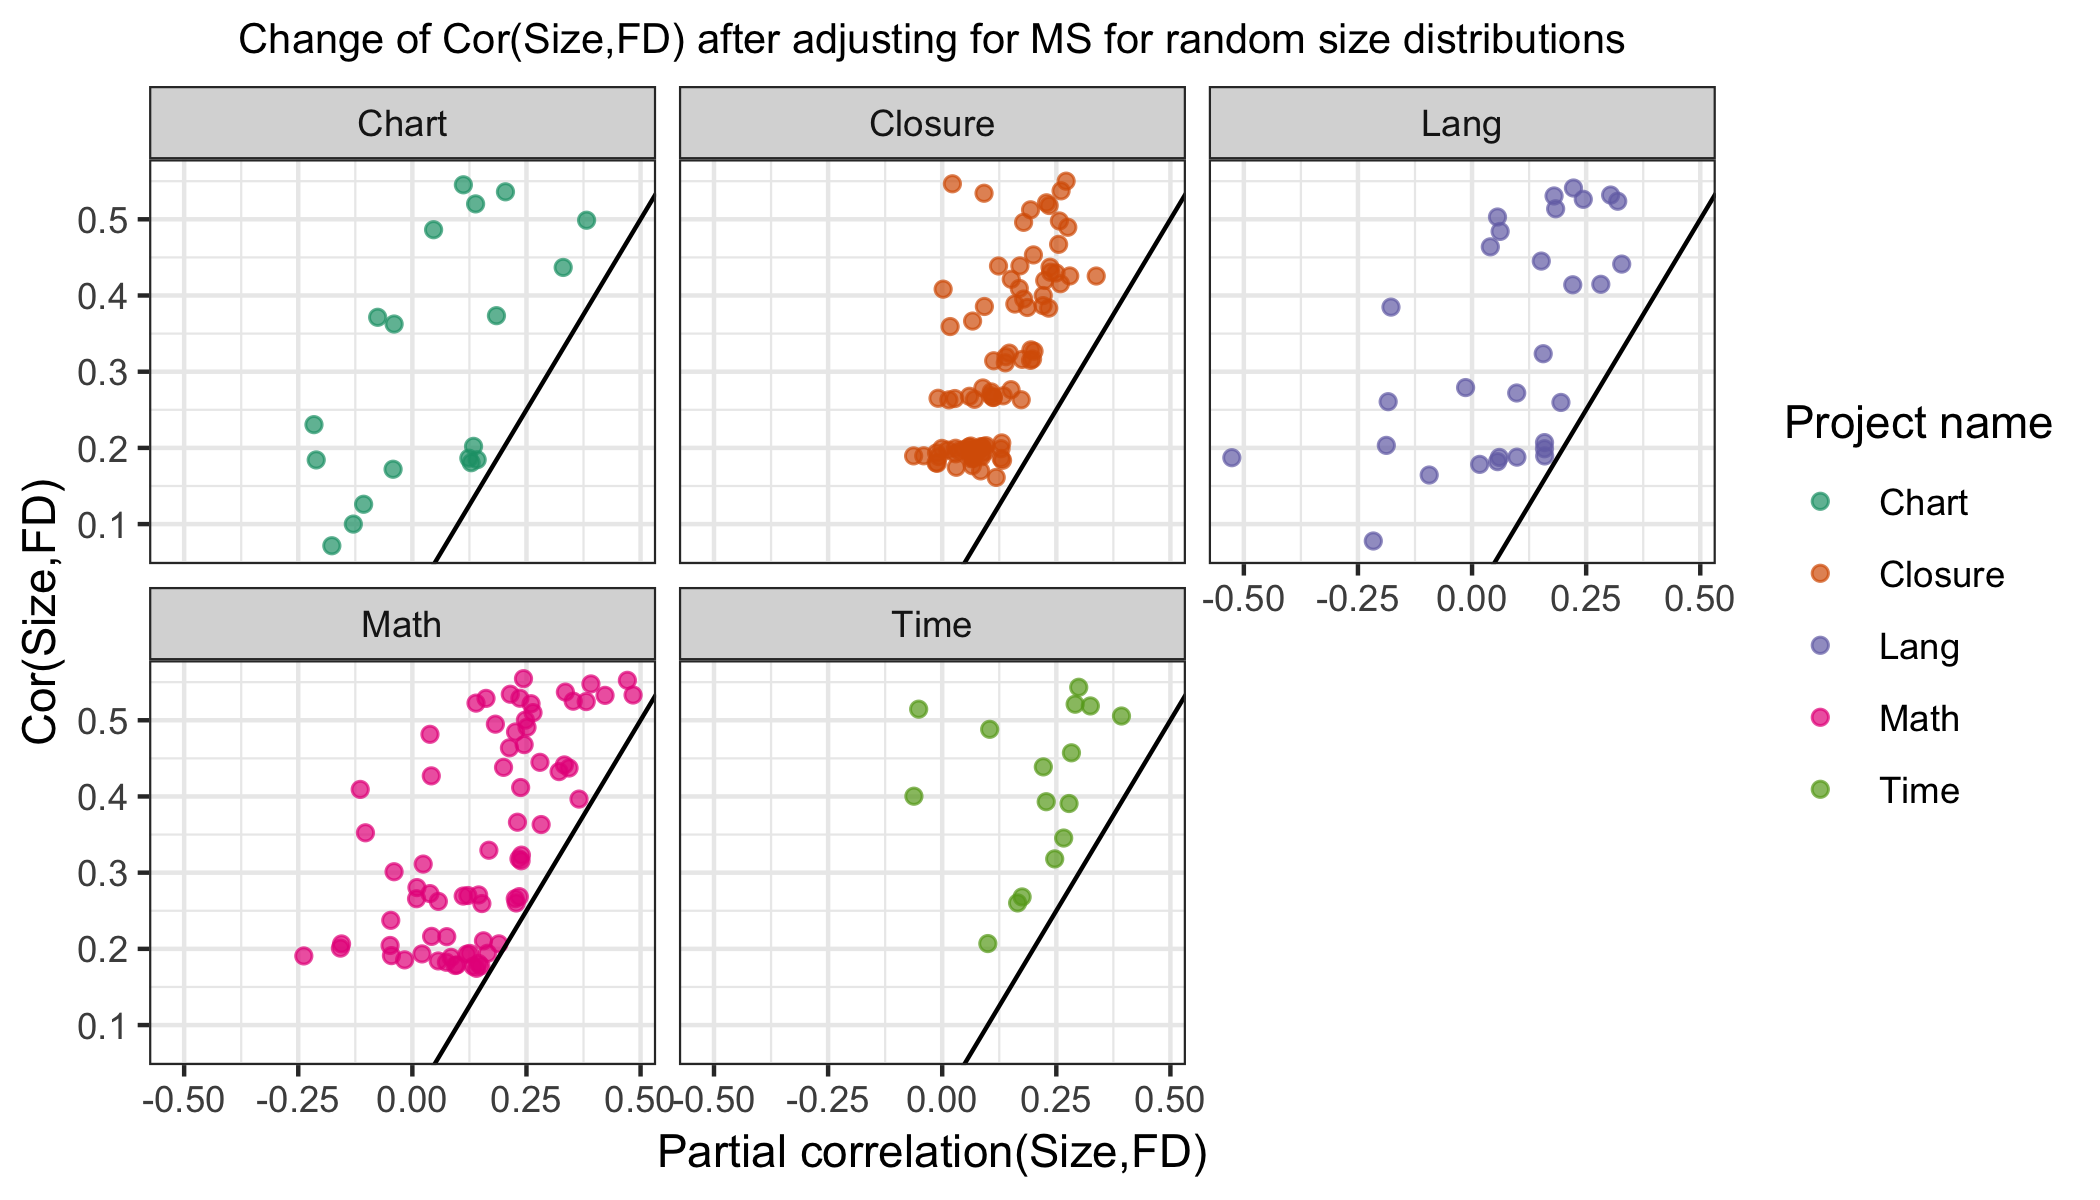
\includegraphics[scale=0.15]{figures/partial_cor_SIZE_fault_scatter.png}
        \caption{Scatter plot of partial correlation (adjusting for mutation score) and correlation between size and fault detection}
        \label{fig:partial_cor_SIZE_fault_scatter}
    \end{figure}

  \begin{figure}[ht!]
        \centering
        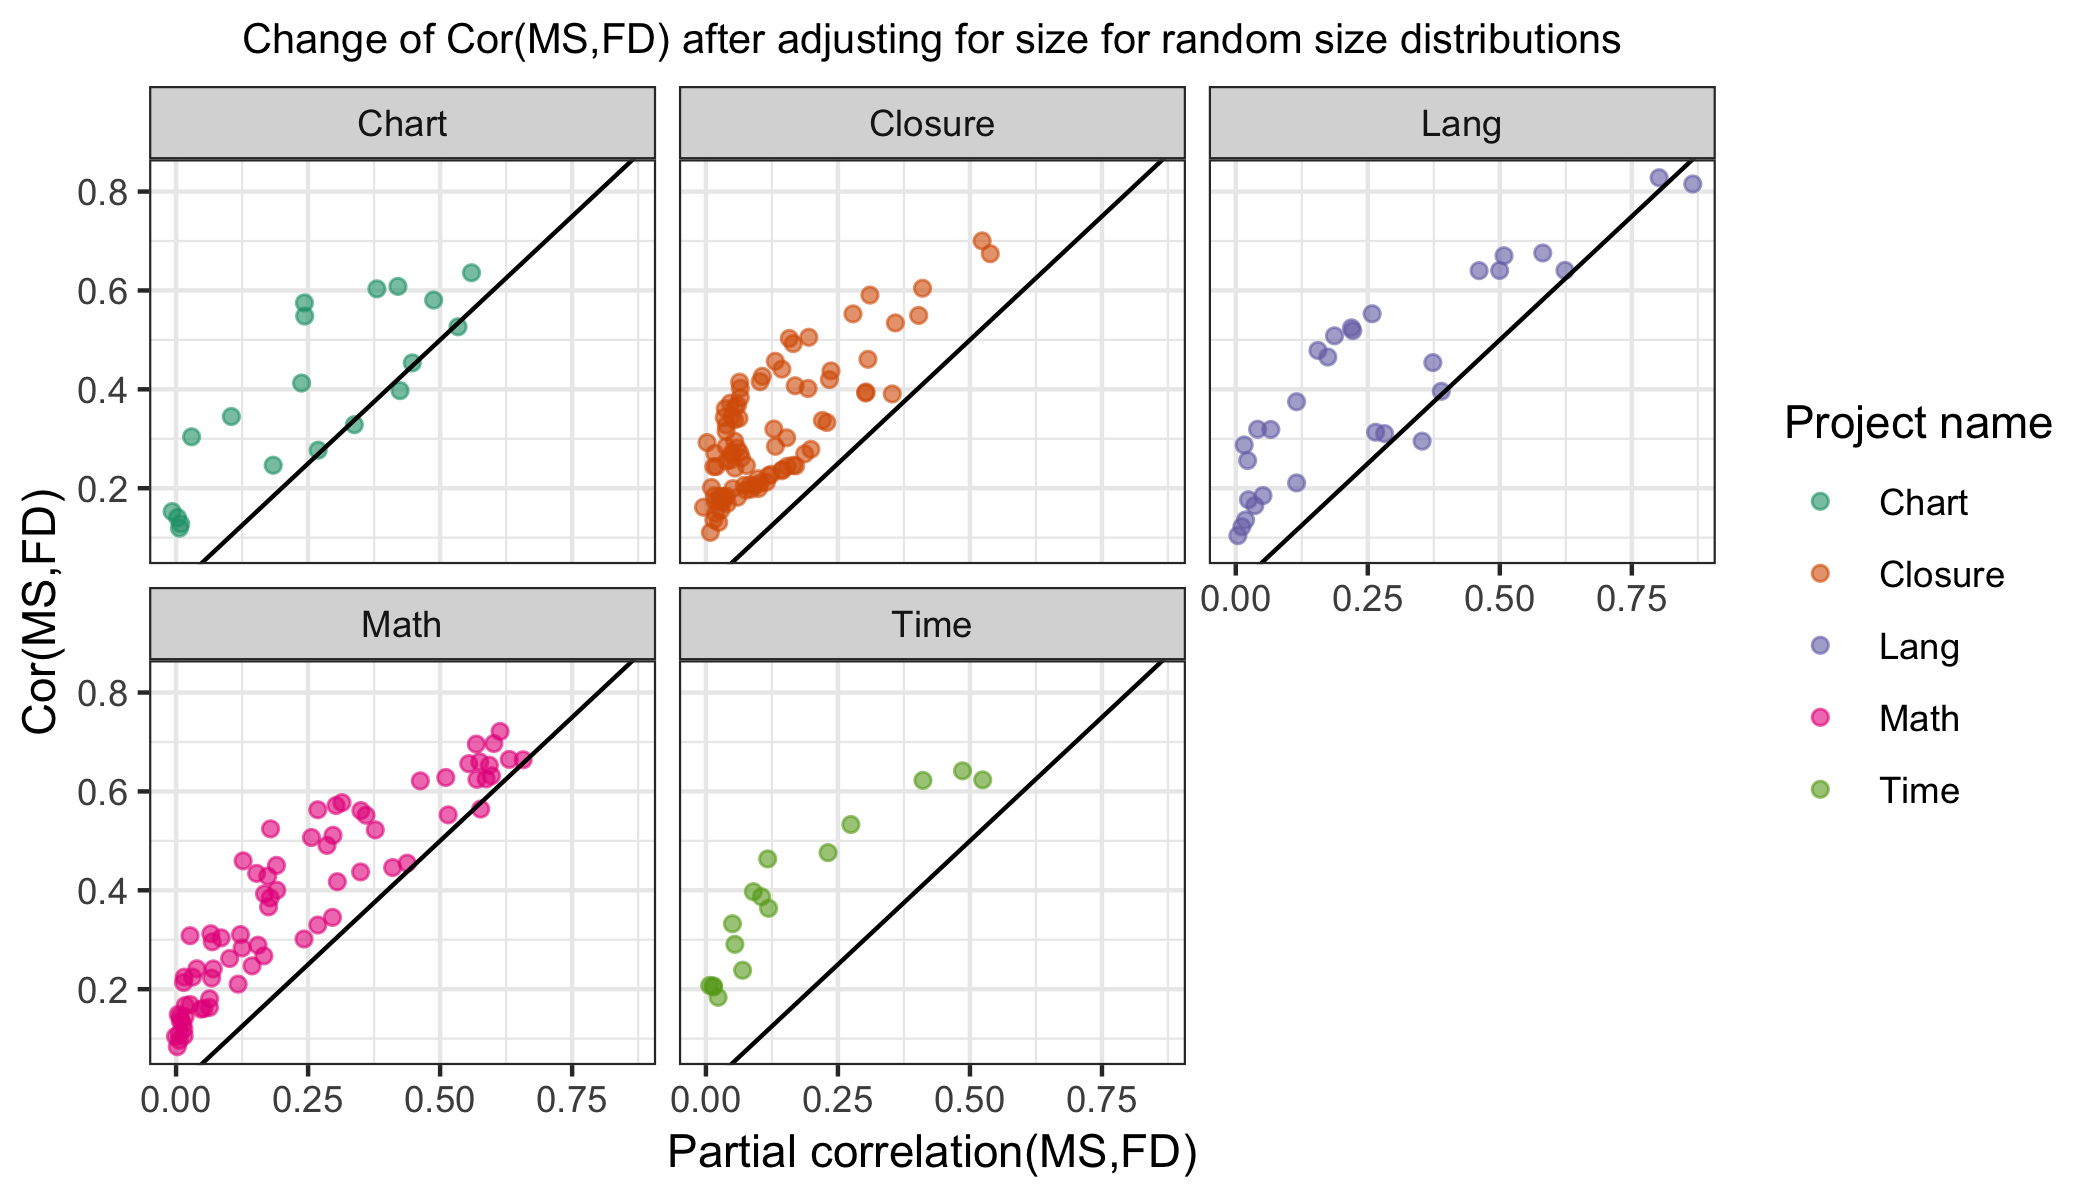
\includegraphics[scale=0.15]{figures/partial_cor_ms_fault_scatter.png}
        \caption{Scatter plot of partial correlation (adjusting for size) and correlation between mutant score and fault detection} 
        \label{fig:partial_cor_ms_fault_scatter}
    \end{figure}



  \begin{figure}[ht!]
        \centering
        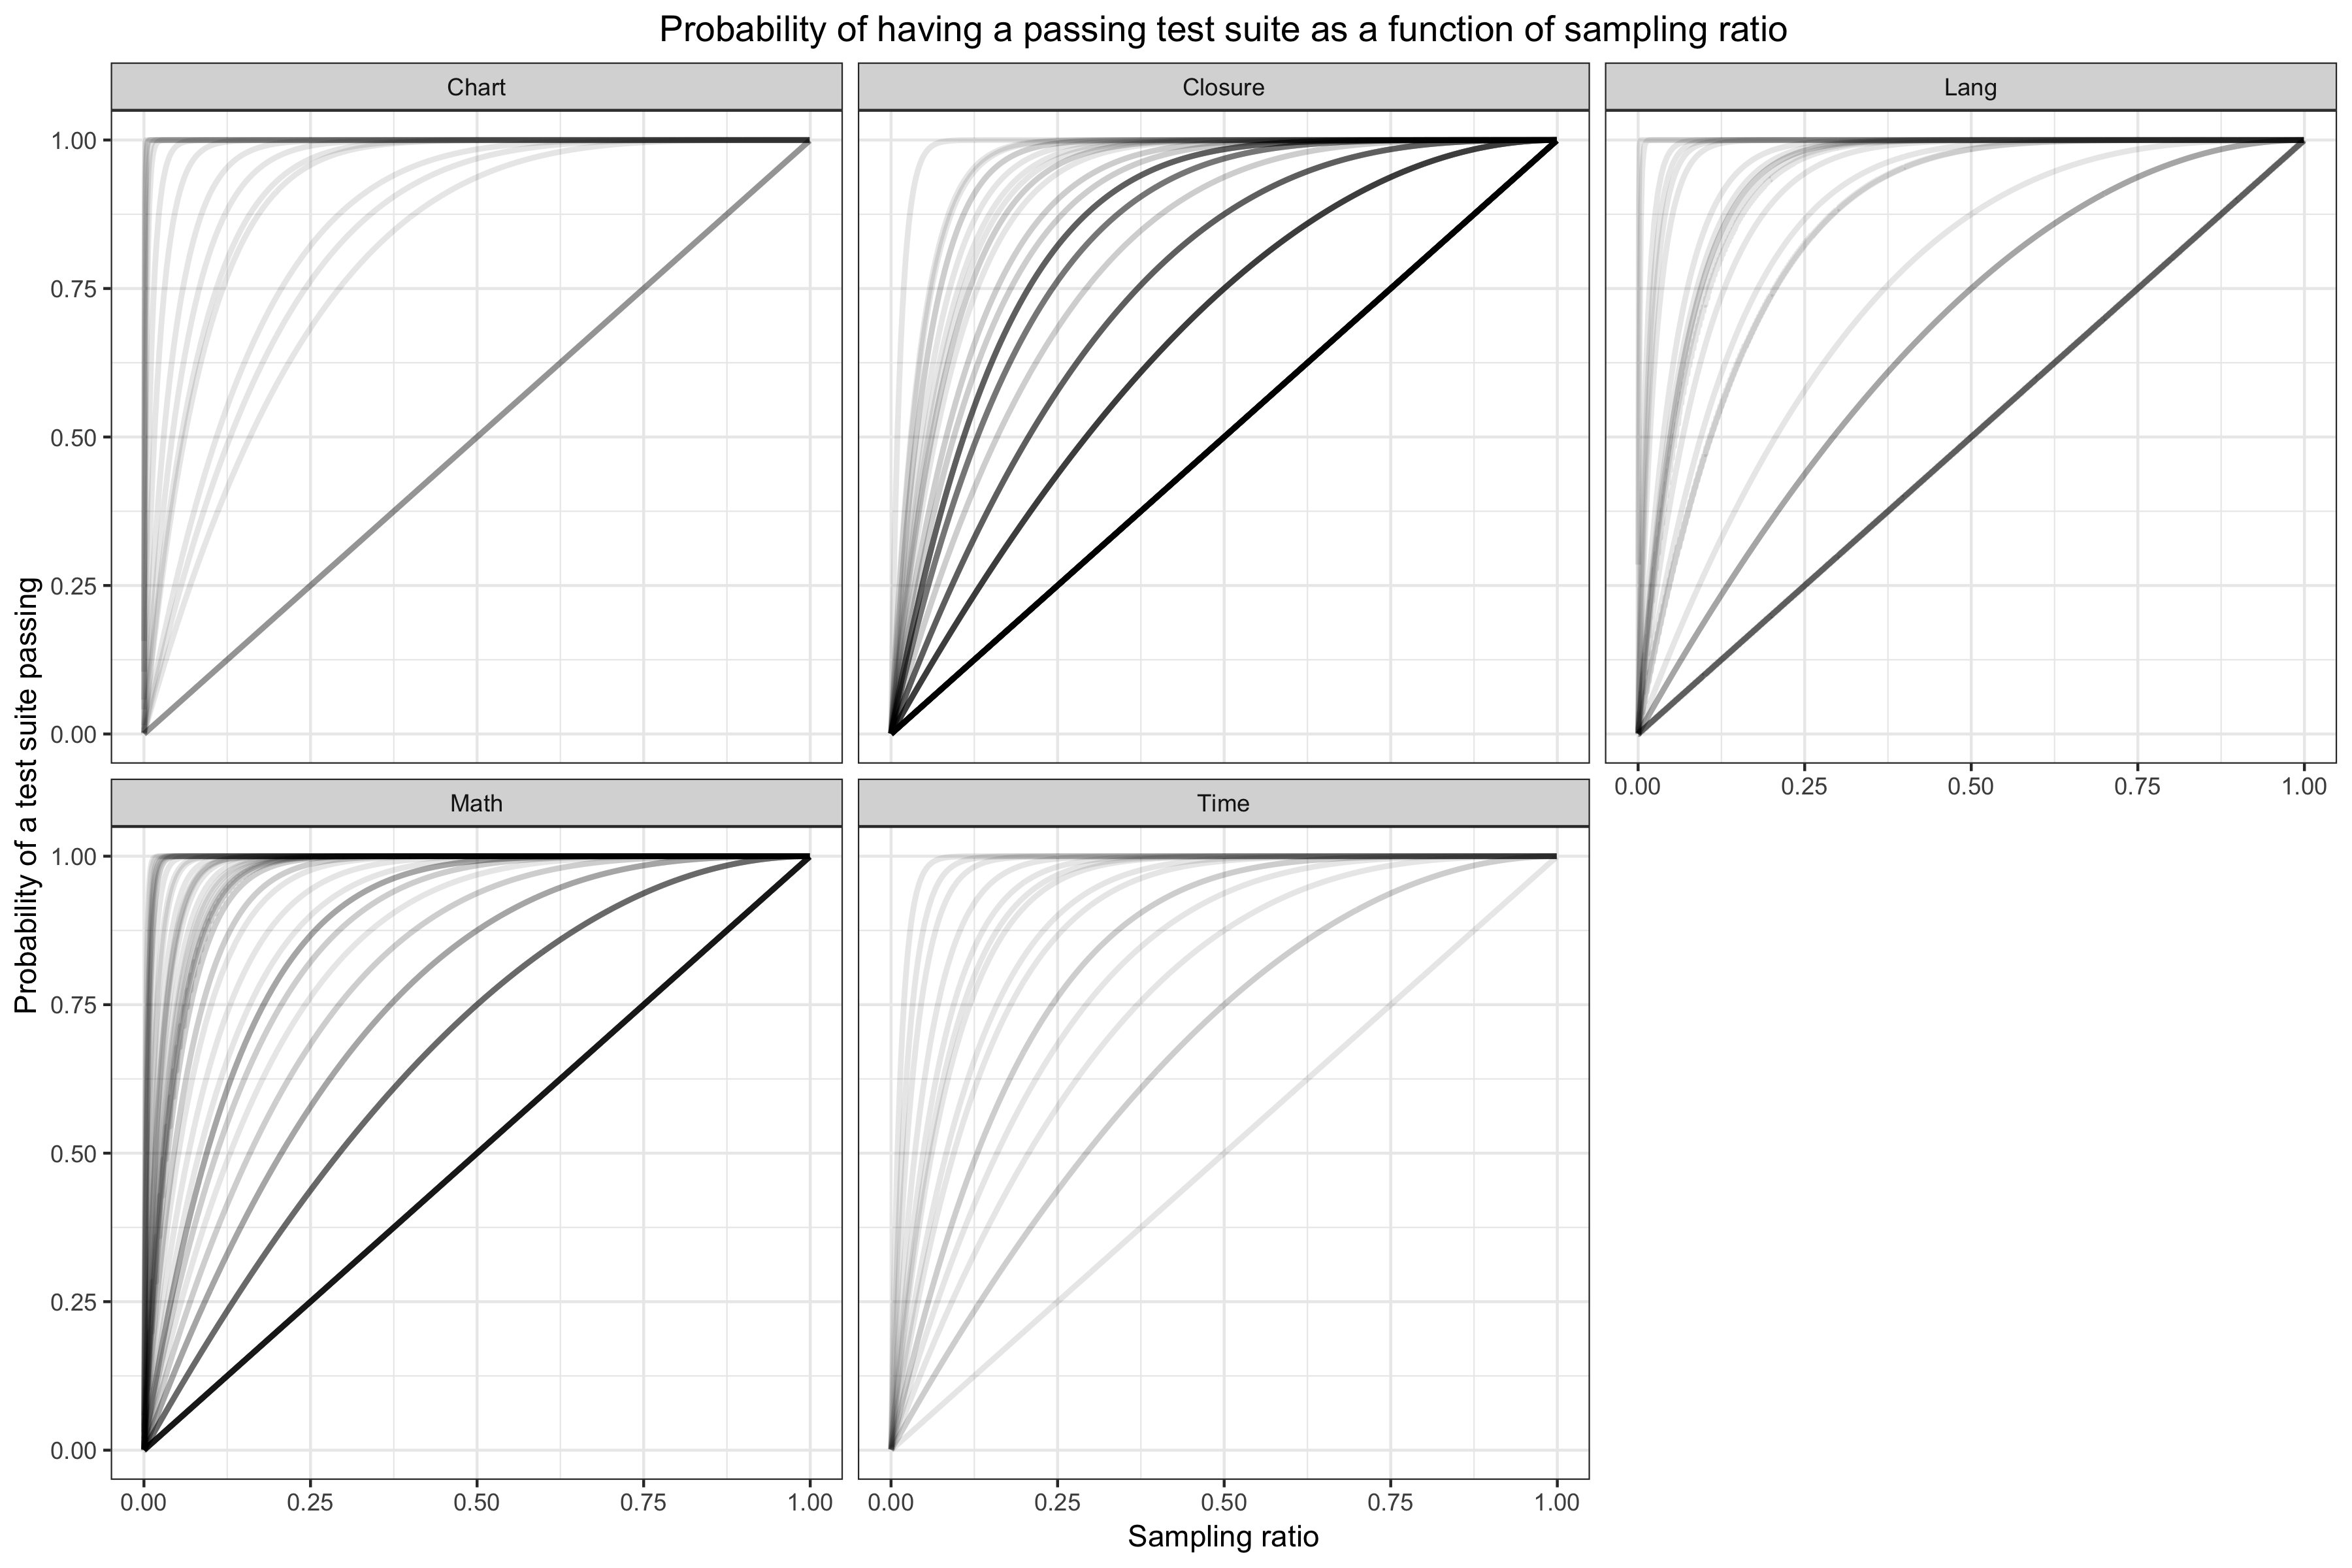
\includegraphics[scale=0.1]{figures/passing_suite_prob.png}
        \caption{Probability of detecting the real fault as a function of sampling ratio, for all 231 Java programs}
        \label{fig:par_cor_ms_fd}
    \end{figure}



  
    \begin{figure}[ht!]
        \centering
        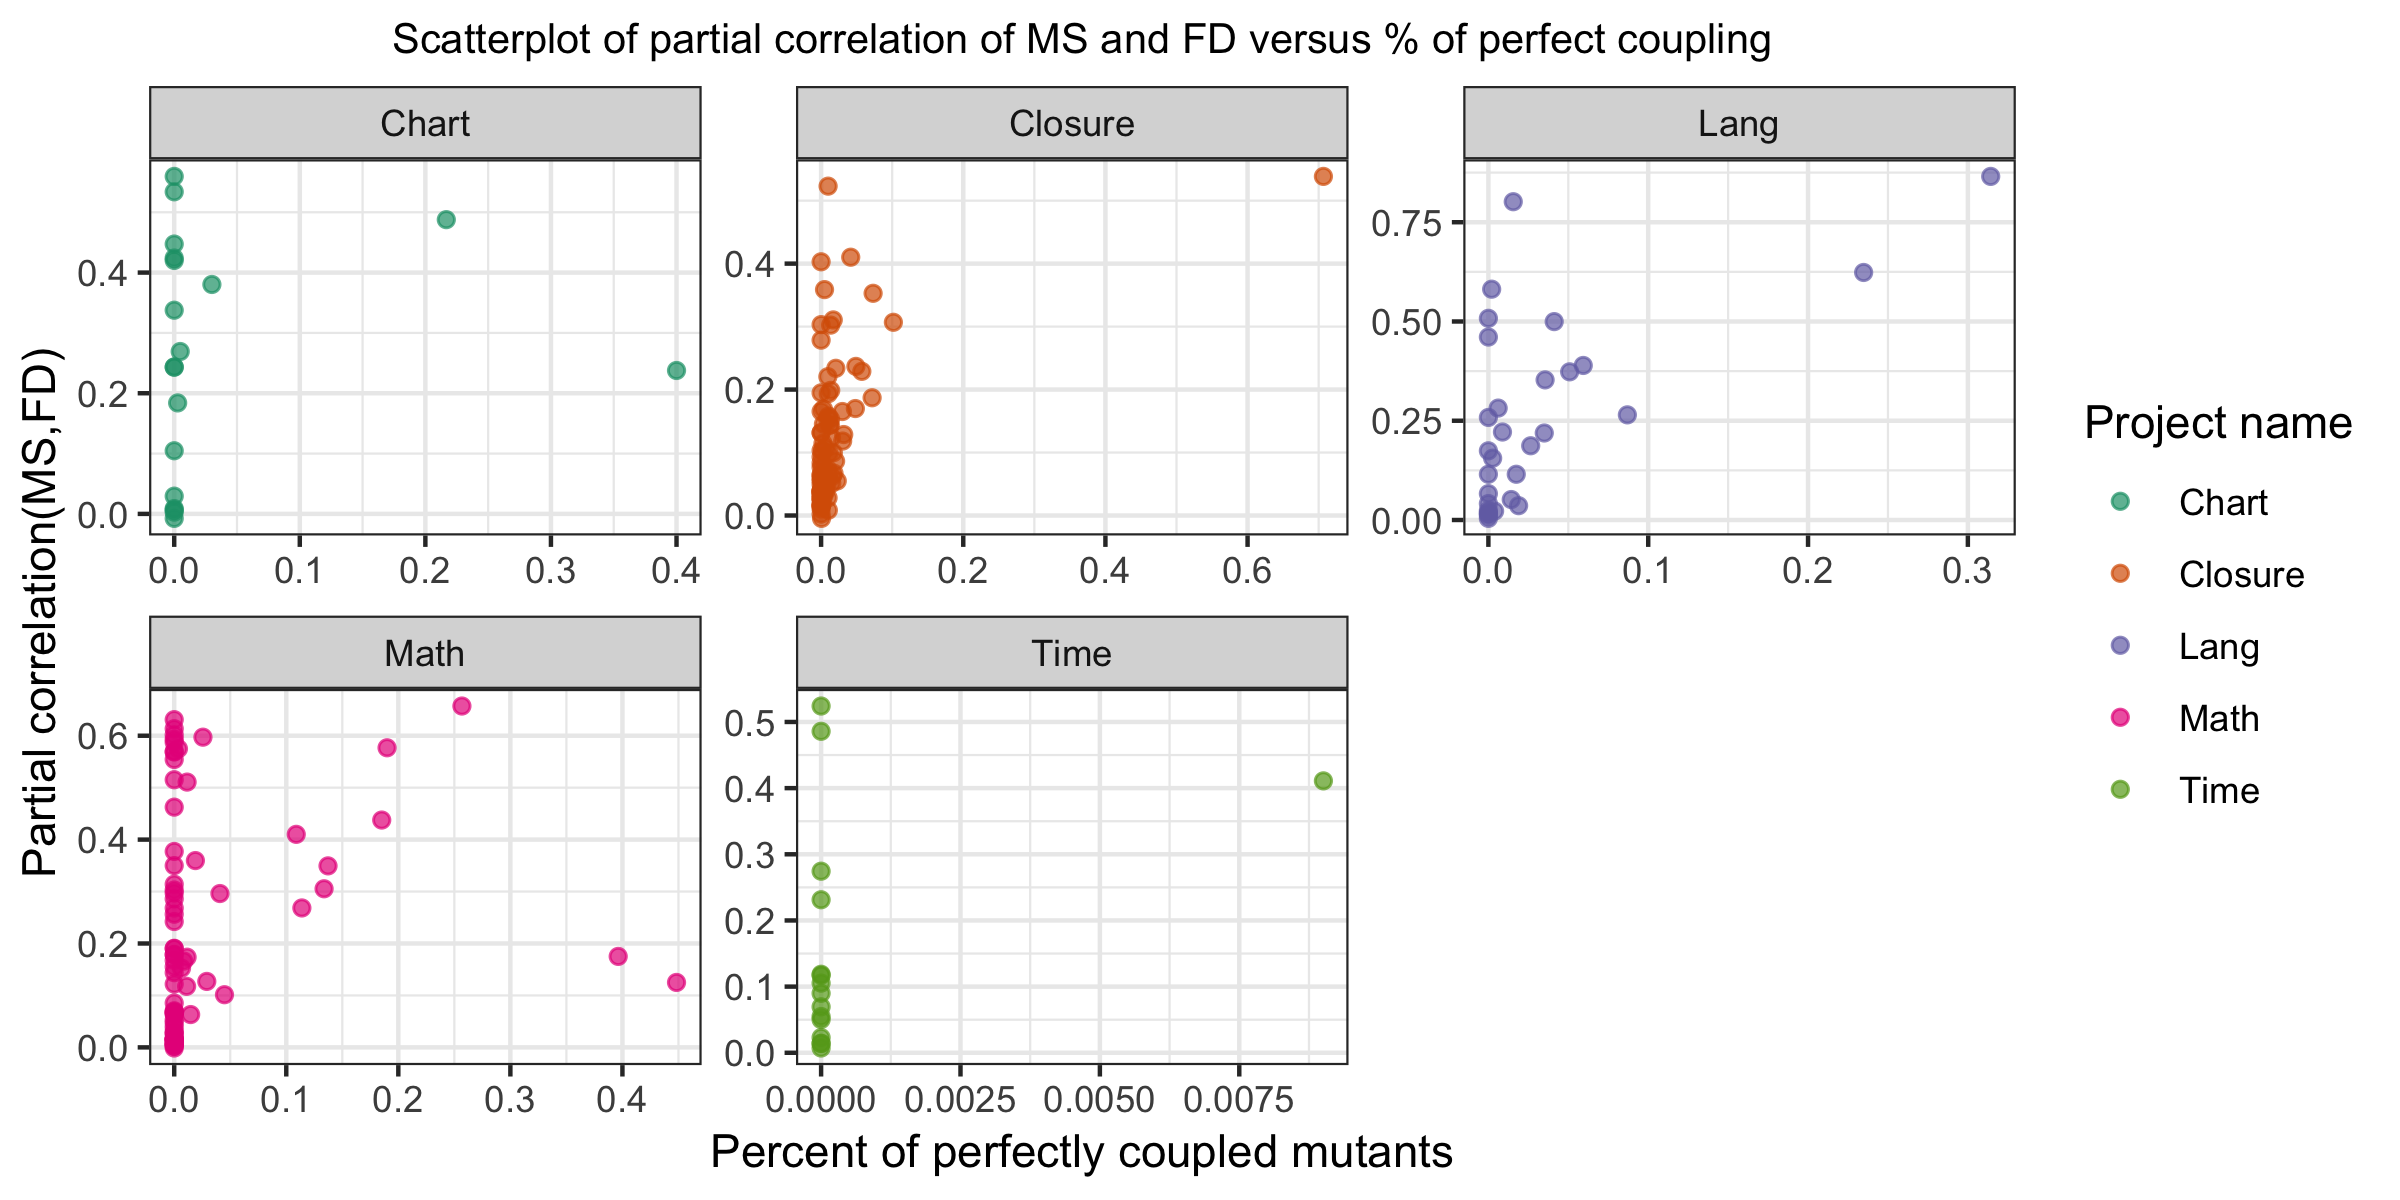
\includegraphics[scale=0.15]{figures/couple_partial_cor.png}
        \caption{Histogram representation of the posterior distribution}
        \label{fig:couple_partial_cor}
    \end{figure}



  \begin{figure}[ht!]
        \centering
        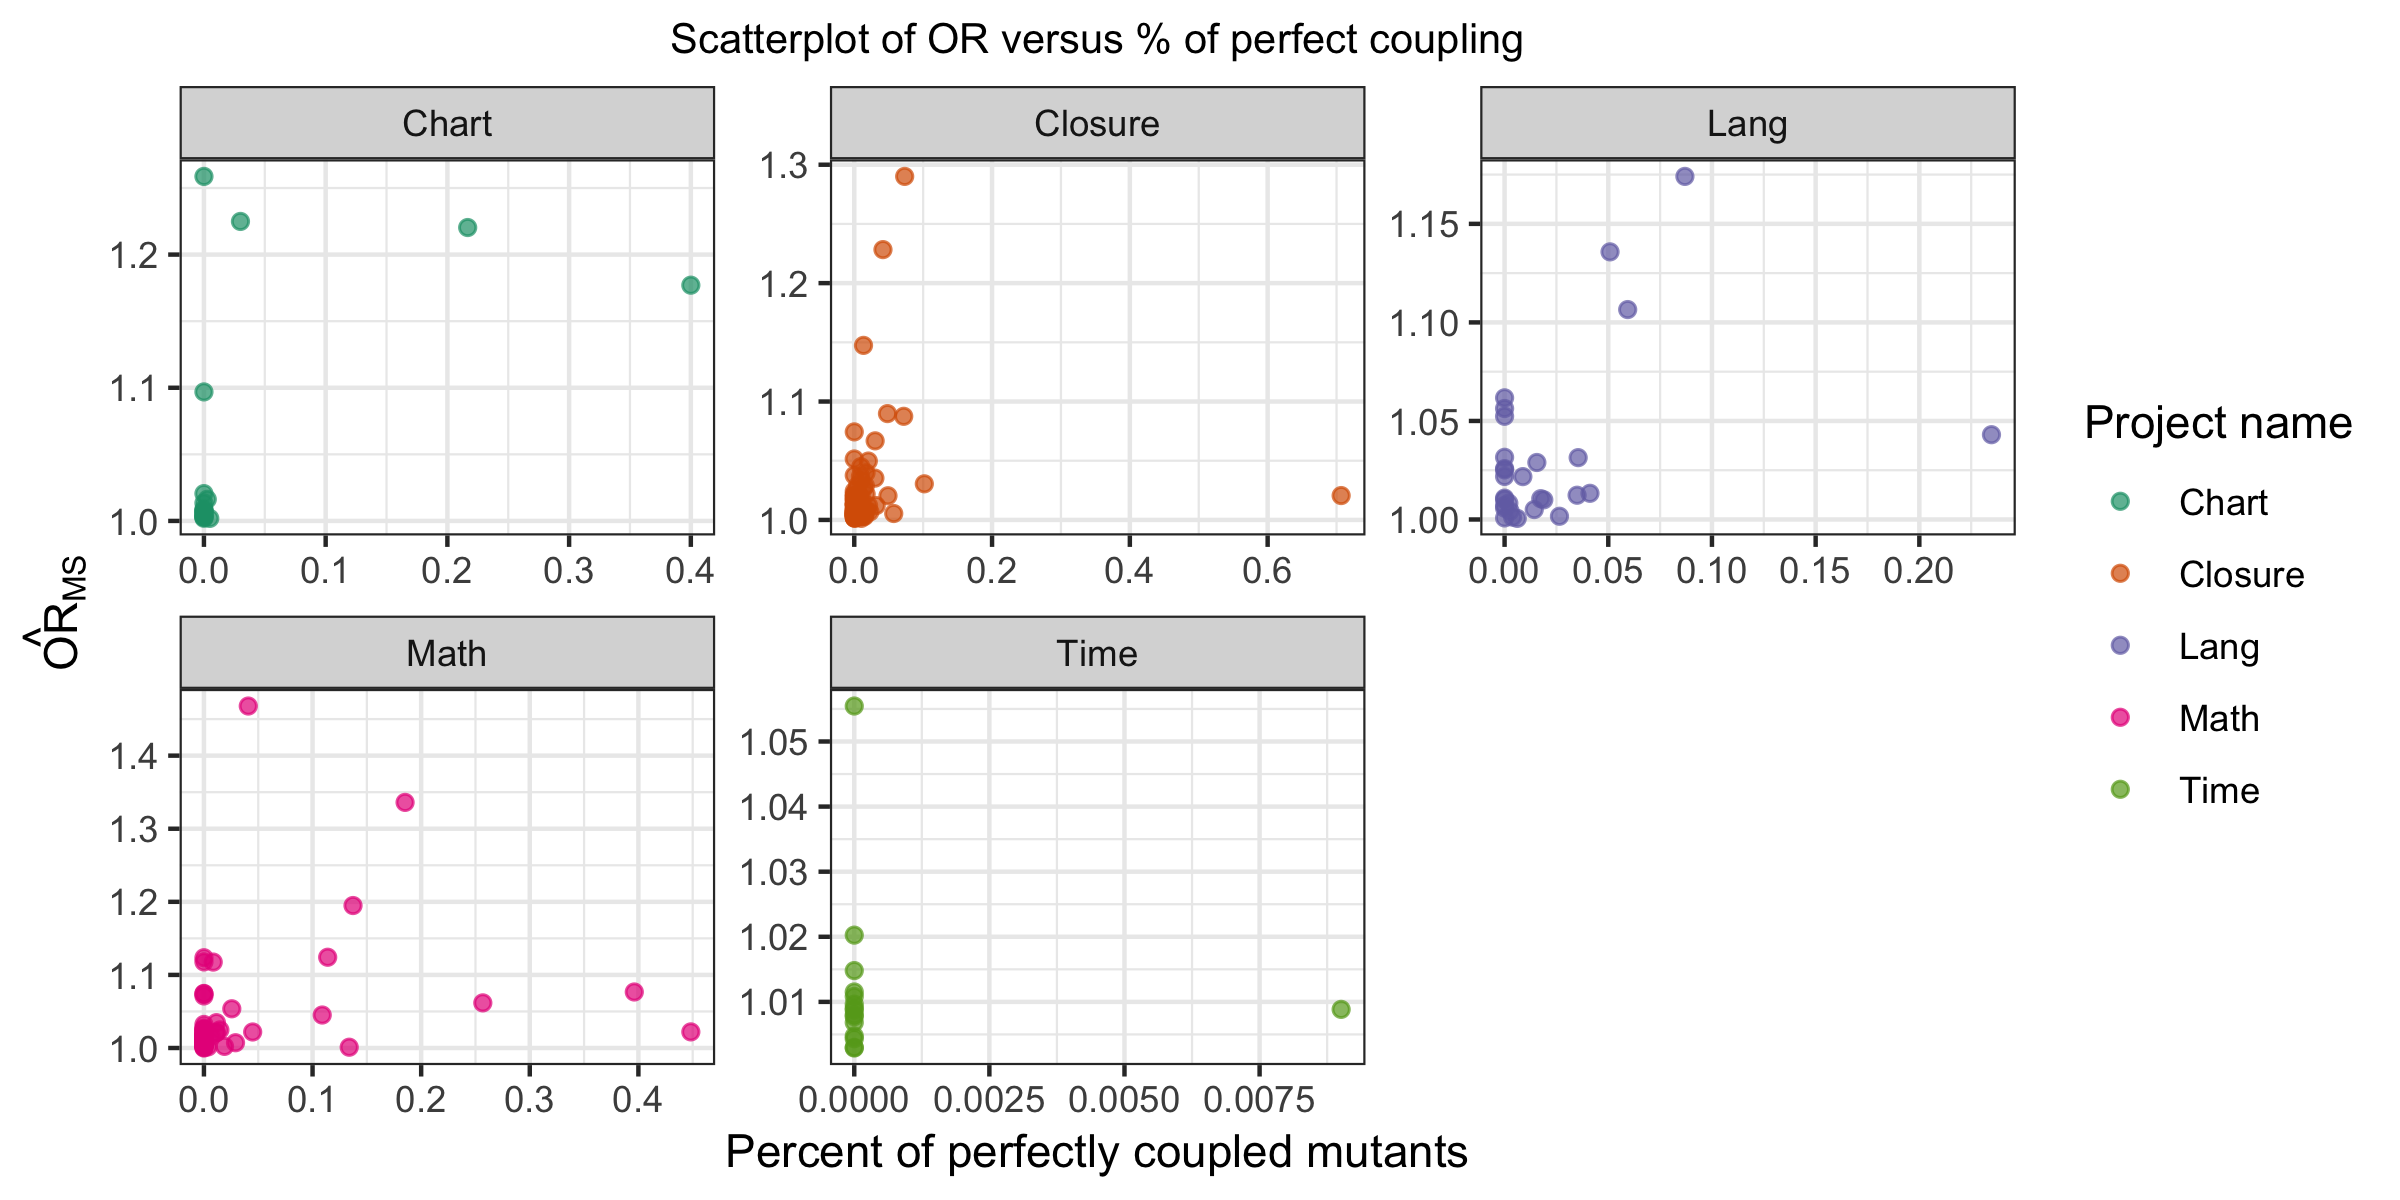
\includegraphics[scale=0.15]{figures/couple_OR.png}
        \caption{Scatter plot of propotion of perfectly coupled mutants and estimated odds ratio }
        \label{fig:couple_OR}
    \end{figure}

%\clearpage
\subsection*{Reference}



%This is where your bibliography is generated. Make sure that your .bib file is actually called library.bib
\bibliography{library}

%This defines the bibliographies style. Search online for a list of available styles.
\bibliographystyle{abbrv}

\end{document}




